%!TEX root = main.tex
\chapter{Lösungen}

\section{Kapitel 1}
\begin{enumerate}
	\item Die Bedeutung ist: Für alle $x$ in der Menge der reellen zahlen existiert ein $y$ sodass die Gleichung stimmt. Die Aussage ist wahr, $y = -x$.
    \item Siehe Abb. \ref{fig:dreiMengenLoes}
    \item 
    \begin{enumerate}
\item Siehe Abb \ref{fig:Loes_min}
\item Siehe Abb \ref{fig:Loes_abs}. Die Bedeutung der Parameter ist durchaus greifbar: die eine Zahl schiebt den Graphen auf und ab, die andere nach links und rechts. Siehe Abb. \ref{fig:Loes_abs_var}.
    \end{enumerate}

\item Eine vielleicht umständliche aber richtige Lösung wäre mit einer Fallunterscheidung:
$$ f(x) = \begin{cases} 
-0.9 & \text{für } x \leq -0.9 \\ 
0.9 & \text{für } x \geq 0.9 \\
x & \text{für }  -0.9 < x < 0.9
\end{cases}$$

Wesentlich eleganter ist aber: $f(x) = min(0.9, max(-0.9, x))$.

\item Zunächst suchen wir einen vernünftigen Wert für $\rho$. Im Internet findet man zb. $7850 kg/m^3$ für Stahl. \\
Die Fläche $A$ muss aus dem Durchmesser der Saite berechnet werden, $A = r^2 \pi$ also $A = \pi (d/2)^2$.  
Schließlich muss die Formel nach $T$ aufgelöst werden:

$$ f_0 = \lambda \sqrt{\frac{T}{\rho A}} \qquad  \Bigm\lvert \cdot \frac{1}{\lambda}$$ 
$$ f_0 \lambda =  \sqrt{\frac{T}{\rho A}} \qquad \Bigm\lvert  \cdot ^2$$
$$ (f_0 \lambda)^2 =  \frac{T}{\rho A} \qquad \Bigm\lvert \cdot \rho A$$
$$ \rho A (f_0 \lambda)^2 =  T $$ 

$\lambda$ ist definiert als $2L$ da die halbe Welle auf der Saite mit der Länge L schwingen kann. $\rho A$ kann vereinfacht werden zu $\mu$, dem Gewicht einer Saite mit Länge $1m$, Durchmesser $d$ dichte $\rho$.

Als Überprüfung der Umformungen/Überlegungen kann man eine Dimensionsanalyse vornehmen: \\

Das gesuchte Ergebnis ist eine Kraft mit Einheit \emph{Newton}. Newton in Basiseinheiten ist wiederum $\frac{kgm}{s^2}$ (siehe $F=ma$). Setzt man die Einheiten für $f$, $\rho$ etc. ein sollte also $\frac{kgm}{s^2}$ herauskommen.\\

$$ \rho [kg/m^3] \cdot A[m^2] (f_0[s^{-1}] \lambda [m])^2 = T \left[\frac{kgm}{s^2}\right]$$

Der Einfachheit halber nur die Einheiten, schrittweise vereinfacht:
$$ kg/m^3  \cdot m^2 (s^{-1} m)^2 = \frac{kgm}{s^2}$$
$$ \frac{kg}{m^3}  \cdot m^2  \frac{m^2}{s^2} = \frac{kgm}{s^2}$$
$$ \frac{kg m^4}{m^3 s^2} = \frac{kgm}{s^2}$$
$$ \frac{kg m}{s^2} = \frac{kgm}{s^2}$$

Die Dimensionsanalyse bestätigt also unsere Gleichung. Mit eingesetzten Werten:
$$A = \pi \left(\frac{0.001}{2}\right)^2 \approx 7.85 \cdot 10^{-7} m^2$$
$$ \mu = A\rho = 7.85 \cdot 10^{-7} m^2 \cdot 7850 kg/m^3 \approx 6.2 \cdot10^{-3} kg/m$$
$$ 6.2\cdot10^{-3}kg/m \cdot(440s^{-1} 1m)^2 \approx \doubleunderline{1200 N}$$

Wenn man nun wissen will welches Gewicht dieser Kraft entspräche kann man durch $g\approx9.8 m/s^2$
 dividieren und bekommt ca $122 kg$.

\item Mittels Gleichung \ref{eq:linearity1} ist es am Einfachsten. Man setzt $A$ negativ, zb $-1$. und bekommt:
$Af(x) = f(Ax) \implies A|x| = |Ax| \to -1\cdot |x| = |-1x|$
Was eine falsche Aussage für alle $x \in \mathbb{R}$ ist!

\end{enumerate}

\begin{figure}[h]
    \centering
    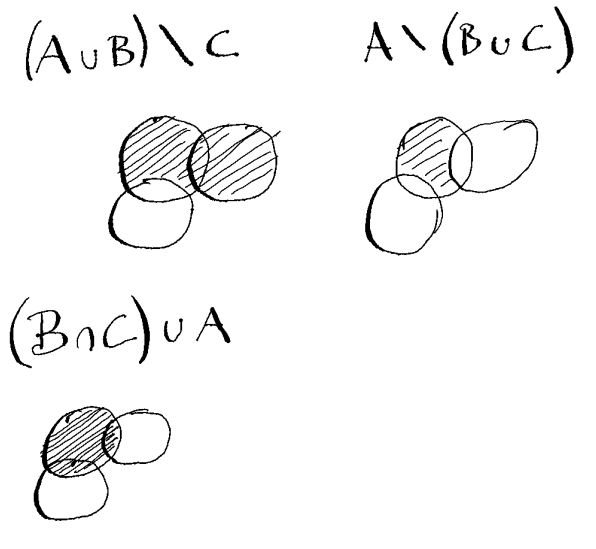
\includegraphics[width=0.3\textwidth]{img/dreiMeingenLoesung.png}
    \caption{Drei Mengen, Lösung. }
    \label{fig:dreiMengenLoes}
\end{figure}

\begin{figure}[h]
    \centering
    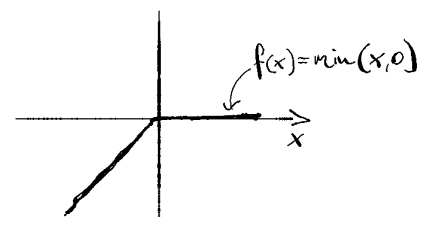
\includegraphics[width=0.3\textwidth]{img/loesung_min.png}
    \caption{Lösung. }
    \label{fig:Loes_min}
\end{figure}

\begin{figure}[h]
    \centering
    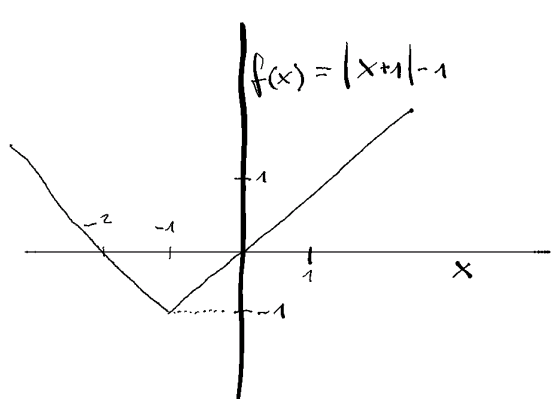
\includegraphics[width=0.3\textwidth]{img/loesung_abs.png}
    \caption{Lösung. }
    \label{fig:Loes_abs}
\end{figure}

\begin{figure}[h]
    \centering
    %% Creator: Matplotlib, PGF backend
%%
%% To include the figure in your LaTeX document, write
%%   \input{<filename>.pgf}
%%
%% Make sure the required packages are loaded in your preamble
%%   \usepackage{pgf}
%%
%% Also ensure that all the required font packages are loaded; for instance,
%% the lmodern package is sometimes necessary when using math font.
%%   \usepackage{lmodern}
%%
%% Figures using additional raster images can only be included by \input if
%% they are in the same directory as the main LaTeX file. For loading figures
%% from other directories you can use the `import` package
%%   \usepackage{import}
%%
%% and then include the figures with
%%   \import{<path to file>}{<filename>.pgf}
%%
%% Matplotlib used the following preamble
%%   \def\mathdefault#1{#1}
%%   \everymath=\expandafter{\the\everymath\displaystyle}
%%   
%%   \usepackage{fontspec}
%%   \setmainfont{VeraSe.ttf}[Path=\detokenize{/usr/share/fonts/TTF/}]
%%   \setsansfont{DejaVuSans.ttf}[Path=\detokenize{/home/pl/miniconda3/lib/python3.12/site-packages/matplotlib/mpl-data/fonts/ttf/}]
%%   \setmonofont{DejaVuSansMono.ttf}[Path=\detokenize{/home/pl/miniconda3/lib/python3.12/site-packages/matplotlib/mpl-data/fonts/ttf/}]
%%   \makeatletter\@ifpackageloaded{underscore}{}{\usepackage[strings]{underscore}}\makeatother
%%
\begingroup%
\makeatletter%
\begin{pgfpicture}%
\pgfpathrectangle{\pgfpointorigin}{\pgfqpoint{5.918612in}{3.167157in}}%
\pgfusepath{use as bounding box, clip}%
\begin{pgfscope}%
\pgfsetbuttcap%
\pgfsetmiterjoin%
\definecolor{currentfill}{rgb}{1.000000,1.000000,1.000000}%
\pgfsetfillcolor{currentfill}%
\pgfsetlinewidth{0.000000pt}%
\definecolor{currentstroke}{rgb}{1.000000,1.000000,1.000000}%
\pgfsetstrokecolor{currentstroke}%
\pgfsetdash{}{0pt}%
\pgfpathmoveto{\pgfqpoint{0.000000in}{0.000000in}}%
\pgfpathlineto{\pgfqpoint{5.918612in}{0.000000in}}%
\pgfpathlineto{\pgfqpoint{5.918612in}{3.167157in}}%
\pgfpathlineto{\pgfqpoint{0.000000in}{3.167157in}}%
\pgfpathlineto{\pgfqpoint{0.000000in}{0.000000in}}%
\pgfpathclose%
\pgfusepath{fill}%
\end{pgfscope}%
\begin{pgfscope}%
\pgfsetbuttcap%
\pgfsetmiterjoin%
\definecolor{currentfill}{rgb}{1.000000,1.000000,1.000000}%
\pgfsetfillcolor{currentfill}%
\pgfsetlinewidth{0.000000pt}%
\definecolor{currentstroke}{rgb}{0.000000,0.000000,0.000000}%
\pgfsetstrokecolor{currentstroke}%
\pgfsetstrokeopacity{0.000000}%
\pgfsetdash{}{0pt}%
\pgfpathmoveto{\pgfqpoint{0.393613in}{0.548486in}}%
\pgfpathlineto{\pgfqpoint{2.859522in}{0.548486in}}%
\pgfpathlineto{\pgfqpoint{2.859522in}{3.014395in}}%
\pgfpathlineto{\pgfqpoint{0.393613in}{3.014395in}}%
\pgfpathlineto{\pgfqpoint{0.393613in}{0.548486in}}%
\pgfpathclose%
\pgfusepath{fill}%
\end{pgfscope}%
\begin{pgfscope}%
\pgfsetbuttcap%
\pgfsetroundjoin%
\definecolor{currentfill}{rgb}{0.000000,0.000000,0.000000}%
\pgfsetfillcolor{currentfill}%
\pgfsetlinewidth{0.803000pt}%
\definecolor{currentstroke}{rgb}{0.000000,0.000000,0.000000}%
\pgfsetstrokecolor{currentstroke}%
\pgfsetdash{}{0pt}%
\pgfsys@defobject{currentmarker}{\pgfqpoint{0.000000in}{-0.048611in}}{\pgfqpoint{0.000000in}{0.000000in}}{%
\pgfpathmoveto{\pgfqpoint{0.000000in}{0.000000in}}%
\pgfpathlineto{\pgfqpoint{0.000000in}{-0.048611in}}%
\pgfusepath{stroke,fill}%
}%
\begin{pgfscope}%
\pgfsys@transformshift{0.804597in}{0.548486in}%
\pgfsys@useobject{currentmarker}{}%
\end{pgfscope}%
\end{pgfscope}%
\begin{pgfscope}%
\definecolor{textcolor}{rgb}{0.000000,0.000000,0.000000}%
\pgfsetstrokecolor{textcolor}%
\pgfsetfillcolor{textcolor}%
\pgftext[x=0.804597in,y=0.451264in,,top]{\color{textcolor}{\rmfamily\fontsize{10.000000}{12.000000}\selectfont\catcode`\^=\active\def^{\ifmmode\sp\else\^{}\fi}\catcode`\%=\active\def%{\%}\ensuremath{-}2}}%
\end{pgfscope}%
\begin{pgfscope}%
\pgfsetbuttcap%
\pgfsetroundjoin%
\definecolor{currentfill}{rgb}{0.000000,0.000000,0.000000}%
\pgfsetfillcolor{currentfill}%
\pgfsetlinewidth{0.803000pt}%
\definecolor{currentstroke}{rgb}{0.000000,0.000000,0.000000}%
\pgfsetstrokecolor{currentstroke}%
\pgfsetdash{}{0pt}%
\pgfsys@defobject{currentmarker}{\pgfqpoint{0.000000in}{-0.048611in}}{\pgfqpoint{0.000000in}{0.000000in}}{%
\pgfpathmoveto{\pgfqpoint{0.000000in}{0.000000in}}%
\pgfpathlineto{\pgfqpoint{0.000000in}{-0.048611in}}%
\pgfusepath{stroke,fill}%
}%
\begin{pgfscope}%
\pgfsys@transformshift{1.626567in}{0.548486in}%
\pgfsys@useobject{currentmarker}{}%
\end{pgfscope}%
\end{pgfscope}%
\begin{pgfscope}%
\definecolor{textcolor}{rgb}{0.000000,0.000000,0.000000}%
\pgfsetstrokecolor{textcolor}%
\pgfsetfillcolor{textcolor}%
\pgftext[x=1.626567in,y=0.451264in,,top]{\color{textcolor}{\rmfamily\fontsize{10.000000}{12.000000}\selectfont\catcode`\^=\active\def^{\ifmmode\sp\else\^{}\fi}\catcode`\%=\active\def%{\%}0}}%
\end{pgfscope}%
\begin{pgfscope}%
\pgfsetbuttcap%
\pgfsetroundjoin%
\definecolor{currentfill}{rgb}{0.000000,0.000000,0.000000}%
\pgfsetfillcolor{currentfill}%
\pgfsetlinewidth{0.803000pt}%
\definecolor{currentstroke}{rgb}{0.000000,0.000000,0.000000}%
\pgfsetstrokecolor{currentstroke}%
\pgfsetdash{}{0pt}%
\pgfsys@defobject{currentmarker}{\pgfqpoint{0.000000in}{-0.048611in}}{\pgfqpoint{0.000000in}{0.000000in}}{%
\pgfpathmoveto{\pgfqpoint{0.000000in}{0.000000in}}%
\pgfpathlineto{\pgfqpoint{0.000000in}{-0.048611in}}%
\pgfusepath{stroke,fill}%
}%
\begin{pgfscope}%
\pgfsys@transformshift{2.448537in}{0.548486in}%
\pgfsys@useobject{currentmarker}{}%
\end{pgfscope}%
\end{pgfscope}%
\begin{pgfscope}%
\definecolor{textcolor}{rgb}{0.000000,0.000000,0.000000}%
\pgfsetstrokecolor{textcolor}%
\pgfsetfillcolor{textcolor}%
\pgftext[x=2.448537in,y=0.451264in,,top]{\color{textcolor}{\rmfamily\fontsize{10.000000}{12.000000}\selectfont\catcode`\^=\active\def^{\ifmmode\sp\else\^{}\fi}\catcode`\%=\active\def%{\%}2}}%
\end{pgfscope}%
\begin{pgfscope}%
\definecolor{textcolor}{rgb}{0.000000,0.000000,0.000000}%
\pgfsetstrokecolor{textcolor}%
\pgfsetfillcolor{textcolor}%
\pgftext[x=1.626567in,y=0.261295in,,top]{\color{textcolor}{\rmfamily\fontsize{12.000000}{14.400000}\selectfont\catcode`\^=\active\def^{\ifmmode\sp\else\^{}\fi}\catcode`\%=\active\def%{\%}$x$}}%
\end{pgfscope}%
\begin{pgfscope}%
\pgfsetbuttcap%
\pgfsetroundjoin%
\definecolor{currentfill}{rgb}{0.000000,0.000000,0.000000}%
\pgfsetfillcolor{currentfill}%
\pgfsetlinewidth{0.803000pt}%
\definecolor{currentstroke}{rgb}{0.000000,0.000000,0.000000}%
\pgfsetstrokecolor{currentstroke}%
\pgfsetdash{}{0pt}%
\pgfsys@defobject{currentmarker}{\pgfqpoint{-0.048611in}{0.000000in}}{\pgfqpoint{-0.000000in}{0.000000in}}{%
\pgfpathmoveto{\pgfqpoint{-0.000000in}{0.000000in}}%
\pgfpathlineto{\pgfqpoint{-0.048611in}{0.000000in}}%
\pgfusepath{stroke,fill}%
}%
\begin{pgfscope}%
\pgfsys@transformshift{0.393613in}{0.548486in}%
\pgfsys@useobject{currentmarker}{}%
\end{pgfscope}%
\end{pgfscope}%
\begin{pgfscope}%
\definecolor{textcolor}{rgb}{0.000000,0.000000,0.000000}%
\pgfsetstrokecolor{textcolor}%
\pgfsetfillcolor{textcolor}%
\pgftext[x=0.100000in, y=0.495724in, left, base]{\color{textcolor}{\rmfamily\fontsize{10.000000}{12.000000}\selectfont\catcode`\^=\active\def^{\ifmmode\sp\else\^{}\fi}\catcode`\%=\active\def%{\%}\ensuremath{-}2}}%
\end{pgfscope}%
\begin{pgfscope}%
\pgfsetbuttcap%
\pgfsetroundjoin%
\definecolor{currentfill}{rgb}{0.000000,0.000000,0.000000}%
\pgfsetfillcolor{currentfill}%
\pgfsetlinewidth{0.803000pt}%
\definecolor{currentstroke}{rgb}{0.000000,0.000000,0.000000}%
\pgfsetstrokecolor{currentstroke}%
\pgfsetdash{}{0pt}%
\pgfsys@defobject{currentmarker}{\pgfqpoint{-0.048611in}{0.000000in}}{\pgfqpoint{-0.000000in}{0.000000in}}{%
\pgfpathmoveto{\pgfqpoint{-0.000000in}{0.000000in}}%
\pgfpathlineto{\pgfqpoint{-0.048611in}{0.000000in}}%
\pgfusepath{stroke,fill}%
}%
\begin{pgfscope}%
\pgfsys@transformshift{0.393613in}{0.959471in}%
\pgfsys@useobject{currentmarker}{}%
\end{pgfscope}%
\end{pgfscope}%
\begin{pgfscope}%
\definecolor{textcolor}{rgb}{0.000000,0.000000,0.000000}%
\pgfsetstrokecolor{textcolor}%
\pgfsetfillcolor{textcolor}%
\pgftext[x=0.100000in, y=0.906709in, left, base]{\color{textcolor}{\rmfamily\fontsize{10.000000}{12.000000}\selectfont\catcode`\^=\active\def^{\ifmmode\sp\else\^{}\fi}\catcode`\%=\active\def%{\%}\ensuremath{-}1}}%
\end{pgfscope}%
\begin{pgfscope}%
\pgfsetbuttcap%
\pgfsetroundjoin%
\definecolor{currentfill}{rgb}{0.000000,0.000000,0.000000}%
\pgfsetfillcolor{currentfill}%
\pgfsetlinewidth{0.803000pt}%
\definecolor{currentstroke}{rgb}{0.000000,0.000000,0.000000}%
\pgfsetstrokecolor{currentstroke}%
\pgfsetdash{}{0pt}%
\pgfsys@defobject{currentmarker}{\pgfqpoint{-0.048611in}{0.000000in}}{\pgfqpoint{-0.000000in}{0.000000in}}{%
\pgfpathmoveto{\pgfqpoint{-0.000000in}{0.000000in}}%
\pgfpathlineto{\pgfqpoint{-0.048611in}{0.000000in}}%
\pgfusepath{stroke,fill}%
}%
\begin{pgfscope}%
\pgfsys@transformshift{0.393613in}{1.370456in}%
\pgfsys@useobject{currentmarker}{}%
\end{pgfscope}%
\end{pgfscope}%
\begin{pgfscope}%
\definecolor{textcolor}{rgb}{0.000000,0.000000,0.000000}%
\pgfsetstrokecolor{textcolor}%
\pgfsetfillcolor{textcolor}%
\pgftext[x=0.208025in, y=1.317694in, left, base]{\color{textcolor}{\rmfamily\fontsize{10.000000}{12.000000}\selectfont\catcode`\^=\active\def^{\ifmmode\sp\else\^{}\fi}\catcode`\%=\active\def%{\%}0}}%
\end{pgfscope}%
\begin{pgfscope}%
\pgfsetbuttcap%
\pgfsetroundjoin%
\definecolor{currentfill}{rgb}{0.000000,0.000000,0.000000}%
\pgfsetfillcolor{currentfill}%
\pgfsetlinewidth{0.803000pt}%
\definecolor{currentstroke}{rgb}{0.000000,0.000000,0.000000}%
\pgfsetstrokecolor{currentstroke}%
\pgfsetdash{}{0pt}%
\pgfsys@defobject{currentmarker}{\pgfqpoint{-0.048611in}{0.000000in}}{\pgfqpoint{-0.000000in}{0.000000in}}{%
\pgfpathmoveto{\pgfqpoint{-0.000000in}{0.000000in}}%
\pgfpathlineto{\pgfqpoint{-0.048611in}{0.000000in}}%
\pgfusepath{stroke,fill}%
}%
\begin{pgfscope}%
\pgfsys@transformshift{0.393613in}{1.781441in}%
\pgfsys@useobject{currentmarker}{}%
\end{pgfscope}%
\end{pgfscope}%
\begin{pgfscope}%
\definecolor{textcolor}{rgb}{0.000000,0.000000,0.000000}%
\pgfsetstrokecolor{textcolor}%
\pgfsetfillcolor{textcolor}%
\pgftext[x=0.208025in, y=1.728679in, left, base]{\color{textcolor}{\rmfamily\fontsize{10.000000}{12.000000}\selectfont\catcode`\^=\active\def^{\ifmmode\sp\else\^{}\fi}\catcode`\%=\active\def%{\%}1}}%
\end{pgfscope}%
\begin{pgfscope}%
\pgfsetbuttcap%
\pgfsetroundjoin%
\definecolor{currentfill}{rgb}{0.000000,0.000000,0.000000}%
\pgfsetfillcolor{currentfill}%
\pgfsetlinewidth{0.803000pt}%
\definecolor{currentstroke}{rgb}{0.000000,0.000000,0.000000}%
\pgfsetstrokecolor{currentstroke}%
\pgfsetdash{}{0pt}%
\pgfsys@defobject{currentmarker}{\pgfqpoint{-0.048611in}{0.000000in}}{\pgfqpoint{-0.000000in}{0.000000in}}{%
\pgfpathmoveto{\pgfqpoint{-0.000000in}{0.000000in}}%
\pgfpathlineto{\pgfqpoint{-0.048611in}{0.000000in}}%
\pgfusepath{stroke,fill}%
}%
\begin{pgfscope}%
\pgfsys@transformshift{0.393613in}{2.192425in}%
\pgfsys@useobject{currentmarker}{}%
\end{pgfscope}%
\end{pgfscope}%
\begin{pgfscope}%
\definecolor{textcolor}{rgb}{0.000000,0.000000,0.000000}%
\pgfsetstrokecolor{textcolor}%
\pgfsetfillcolor{textcolor}%
\pgftext[x=0.208025in, y=2.139664in, left, base]{\color{textcolor}{\rmfamily\fontsize{10.000000}{12.000000}\selectfont\catcode`\^=\active\def^{\ifmmode\sp\else\^{}\fi}\catcode`\%=\active\def%{\%}2}}%
\end{pgfscope}%
\begin{pgfscope}%
\pgfsetbuttcap%
\pgfsetroundjoin%
\definecolor{currentfill}{rgb}{0.000000,0.000000,0.000000}%
\pgfsetfillcolor{currentfill}%
\pgfsetlinewidth{0.803000pt}%
\definecolor{currentstroke}{rgb}{0.000000,0.000000,0.000000}%
\pgfsetstrokecolor{currentstroke}%
\pgfsetdash{}{0pt}%
\pgfsys@defobject{currentmarker}{\pgfqpoint{-0.048611in}{0.000000in}}{\pgfqpoint{-0.000000in}{0.000000in}}{%
\pgfpathmoveto{\pgfqpoint{-0.000000in}{0.000000in}}%
\pgfpathlineto{\pgfqpoint{-0.048611in}{0.000000in}}%
\pgfusepath{stroke,fill}%
}%
\begin{pgfscope}%
\pgfsys@transformshift{0.393613in}{2.603410in}%
\pgfsys@useobject{currentmarker}{}%
\end{pgfscope}%
\end{pgfscope}%
\begin{pgfscope}%
\definecolor{textcolor}{rgb}{0.000000,0.000000,0.000000}%
\pgfsetstrokecolor{textcolor}%
\pgfsetfillcolor{textcolor}%
\pgftext[x=0.208025in, y=2.550649in, left, base]{\color{textcolor}{\rmfamily\fontsize{10.000000}{12.000000}\selectfont\catcode`\^=\active\def^{\ifmmode\sp\else\^{}\fi}\catcode`\%=\active\def%{\%}3}}%
\end{pgfscope}%
\begin{pgfscope}%
\pgfsetbuttcap%
\pgfsetroundjoin%
\definecolor{currentfill}{rgb}{0.000000,0.000000,0.000000}%
\pgfsetfillcolor{currentfill}%
\pgfsetlinewidth{0.803000pt}%
\definecolor{currentstroke}{rgb}{0.000000,0.000000,0.000000}%
\pgfsetstrokecolor{currentstroke}%
\pgfsetdash{}{0pt}%
\pgfsys@defobject{currentmarker}{\pgfqpoint{-0.048611in}{0.000000in}}{\pgfqpoint{-0.000000in}{0.000000in}}{%
\pgfpathmoveto{\pgfqpoint{-0.000000in}{0.000000in}}%
\pgfpathlineto{\pgfqpoint{-0.048611in}{0.000000in}}%
\pgfusepath{stroke,fill}%
}%
\begin{pgfscope}%
\pgfsys@transformshift{0.393613in}{3.014395in}%
\pgfsys@useobject{currentmarker}{}%
\end{pgfscope}%
\end{pgfscope}%
\begin{pgfscope}%
\definecolor{textcolor}{rgb}{0.000000,0.000000,0.000000}%
\pgfsetstrokecolor{textcolor}%
\pgfsetfillcolor{textcolor}%
\pgftext[x=0.208025in, y=2.961634in, left, base]{\color{textcolor}{\rmfamily\fontsize{10.000000}{12.000000}\selectfont\catcode`\^=\active\def^{\ifmmode\sp\else\^{}\fi}\catcode`\%=\active\def%{\%}4}}%
\end{pgfscope}%
\begin{pgfscope}%
\pgfpathrectangle{\pgfqpoint{0.393613in}{0.548486in}}{\pgfqpoint{2.465909in}{2.465909in}}%
\pgfusepath{clip}%
\pgfsetrectcap%
\pgfsetroundjoin%
\pgfsetlinewidth{1.505625pt}%
\definecolor{currentstroke}{rgb}{0.000000,0.000000,0.000000}%
\pgfsetstrokecolor{currentstroke}%
\pgfsetdash{}{0pt}%
\pgfpathmoveto{\pgfqpoint{0.393613in}{3.014395in}}%
\pgfpathlineto{\pgfqpoint{0.418521in}{2.989487in}}%
\pgfpathlineto{\pgfqpoint{0.443429in}{2.964579in}}%
\pgfpathlineto{\pgfqpoint{0.468337in}{2.939671in}}%
\pgfpathlineto{\pgfqpoint{0.493245in}{2.914762in}}%
\pgfpathlineto{\pgfqpoint{0.518153in}{2.889854in}}%
\pgfpathlineto{\pgfqpoint{0.543062in}{2.864946in}}%
\pgfpathlineto{\pgfqpoint{0.567970in}{2.840038in}}%
\pgfpathlineto{\pgfqpoint{0.592878in}{2.815130in}}%
\pgfpathlineto{\pgfqpoint{0.617786in}{2.790222in}}%
\pgfpathlineto{\pgfqpoint{0.642694in}{2.765313in}}%
\pgfpathlineto{\pgfqpoint{0.667602in}{2.740405in}}%
\pgfpathlineto{\pgfqpoint{0.692511in}{2.715497in}}%
\pgfpathlineto{\pgfqpoint{0.717419in}{2.690589in}}%
\pgfpathlineto{\pgfqpoint{0.742327in}{2.665681in}}%
\pgfpathlineto{\pgfqpoint{0.767235in}{2.640772in}}%
\pgfpathlineto{\pgfqpoint{0.792143in}{2.615864in}}%
\pgfpathlineto{\pgfqpoint{0.817051in}{2.590956in}}%
\pgfpathlineto{\pgfqpoint{0.841960in}{2.566048in}}%
\pgfpathlineto{\pgfqpoint{0.866868in}{2.541140in}}%
\pgfpathlineto{\pgfqpoint{0.891776in}{2.516232in}}%
\pgfpathlineto{\pgfqpoint{0.916684in}{2.491323in}}%
\pgfpathlineto{\pgfqpoint{0.941592in}{2.466415in}}%
\pgfpathlineto{\pgfqpoint{0.966500in}{2.441507in}}%
\pgfpathlineto{\pgfqpoint{0.991409in}{2.416599in}}%
\pgfpathlineto{\pgfqpoint{1.016317in}{2.391691in}}%
\pgfpathlineto{\pgfqpoint{1.041225in}{2.366783in}}%
\pgfpathlineto{\pgfqpoint{1.066133in}{2.341874in}}%
\pgfpathlineto{\pgfqpoint{1.091041in}{2.316966in}}%
\pgfpathlineto{\pgfqpoint{1.115950in}{2.292058in}}%
\pgfpathlineto{\pgfqpoint{1.140858in}{2.267150in}}%
\pgfpathlineto{\pgfqpoint{1.165766in}{2.242242in}}%
\pgfpathlineto{\pgfqpoint{1.190674in}{2.217334in}}%
\pgfpathlineto{\pgfqpoint{1.215582in}{2.192425in}}%
\pgfpathlineto{\pgfqpoint{1.240490in}{2.167517in}}%
\pgfpathlineto{\pgfqpoint{1.265399in}{2.142609in}}%
\pgfpathlineto{\pgfqpoint{1.290307in}{2.117701in}}%
\pgfpathlineto{\pgfqpoint{1.315215in}{2.092793in}}%
\pgfpathlineto{\pgfqpoint{1.340123in}{2.067885in}}%
\pgfpathlineto{\pgfqpoint{1.365031in}{2.042976in}}%
\pgfpathlineto{\pgfqpoint{1.389939in}{2.018068in}}%
\pgfpathlineto{\pgfqpoint{1.414848in}{1.993160in}}%
\pgfpathlineto{\pgfqpoint{1.439756in}{1.968252in}}%
\pgfpathlineto{\pgfqpoint{1.464664in}{1.943344in}}%
\pgfpathlineto{\pgfqpoint{1.489572in}{1.918435in}}%
\pgfpathlineto{\pgfqpoint{1.514480in}{1.893527in}}%
\pgfpathlineto{\pgfqpoint{1.539388in}{1.868619in}}%
\pgfpathlineto{\pgfqpoint{1.564297in}{1.843711in}}%
\pgfpathlineto{\pgfqpoint{1.589205in}{1.818803in}}%
\pgfpathlineto{\pgfqpoint{1.614113in}{1.793895in}}%
\pgfpathlineto{\pgfqpoint{1.639021in}{1.768986in}}%
\pgfpathlineto{\pgfqpoint{1.663929in}{1.744078in}}%
\pgfpathlineto{\pgfqpoint{1.688837in}{1.719170in}}%
\pgfpathlineto{\pgfqpoint{1.713746in}{1.694262in}}%
\pgfpathlineto{\pgfqpoint{1.738654in}{1.669354in}}%
\pgfpathlineto{\pgfqpoint{1.763562in}{1.644446in}}%
\pgfpathlineto{\pgfqpoint{1.788470in}{1.619537in}}%
\pgfpathlineto{\pgfqpoint{1.813378in}{1.594629in}}%
\pgfpathlineto{\pgfqpoint{1.838287in}{1.569721in}}%
\pgfpathlineto{\pgfqpoint{1.863195in}{1.544813in}}%
\pgfpathlineto{\pgfqpoint{1.888103in}{1.519905in}}%
\pgfpathlineto{\pgfqpoint{1.913011in}{1.494997in}}%
\pgfpathlineto{\pgfqpoint{1.937919in}{1.470088in}}%
\pgfpathlineto{\pgfqpoint{1.962827in}{1.445180in}}%
\pgfpathlineto{\pgfqpoint{1.987736in}{1.420272in}}%
\pgfpathlineto{\pgfqpoint{2.012644in}{1.395364in}}%
\pgfpathlineto{\pgfqpoint{2.037552in}{1.370456in}}%
\pgfpathlineto{\pgfqpoint{2.062460in}{1.345547in}}%
\pgfpathlineto{\pgfqpoint{2.087368in}{1.320639in}}%
\pgfpathlineto{\pgfqpoint{2.112276in}{1.295731in}}%
\pgfpathlineto{\pgfqpoint{2.137185in}{1.270823in}}%
\pgfpathlineto{\pgfqpoint{2.162093in}{1.245915in}}%
\pgfpathlineto{\pgfqpoint{2.187001in}{1.221007in}}%
\pgfpathlineto{\pgfqpoint{2.211909in}{1.196098in}}%
\pgfpathlineto{\pgfqpoint{2.236817in}{1.171190in}}%
\pgfpathlineto{\pgfqpoint{2.261725in}{1.146282in}}%
\pgfpathlineto{\pgfqpoint{2.286634in}{1.121374in}}%
\pgfpathlineto{\pgfqpoint{2.311542in}{1.096466in}}%
\pgfpathlineto{\pgfqpoint{2.336450in}{1.071558in}}%
\pgfpathlineto{\pgfqpoint{2.361358in}{1.046649in}}%
\pgfpathlineto{\pgfqpoint{2.386266in}{1.021741in}}%
\pgfpathlineto{\pgfqpoint{2.411174in}{0.996833in}}%
\pgfpathlineto{\pgfqpoint{2.436083in}{0.971925in}}%
\pgfpathlineto{\pgfqpoint{2.460991in}{0.971925in}}%
\pgfpathlineto{\pgfqpoint{2.485899in}{0.996833in}}%
\pgfpathlineto{\pgfqpoint{2.510807in}{1.021741in}}%
\pgfpathlineto{\pgfqpoint{2.535715in}{1.046649in}}%
\pgfpathlineto{\pgfqpoint{2.560624in}{1.071558in}}%
\pgfpathlineto{\pgfqpoint{2.585532in}{1.096466in}}%
\pgfpathlineto{\pgfqpoint{2.610440in}{1.121374in}}%
\pgfpathlineto{\pgfqpoint{2.635348in}{1.146282in}}%
\pgfpathlineto{\pgfqpoint{2.660256in}{1.171190in}}%
\pgfpathlineto{\pgfqpoint{2.685164in}{1.196098in}}%
\pgfpathlineto{\pgfqpoint{2.710073in}{1.221007in}}%
\pgfpathlineto{\pgfqpoint{2.734981in}{1.245915in}}%
\pgfpathlineto{\pgfqpoint{2.759889in}{1.270823in}}%
\pgfpathlineto{\pgfqpoint{2.784797in}{1.295731in}}%
\pgfpathlineto{\pgfqpoint{2.809705in}{1.320639in}}%
\pgfpathlineto{\pgfqpoint{2.834613in}{1.345547in}}%
\pgfpathlineto{\pgfqpoint{2.859522in}{1.370456in}}%
\pgfusepath{stroke}%
\end{pgfscope}%
\begin{pgfscope}%
\pgfpathrectangle{\pgfqpoint{0.393613in}{0.548486in}}{\pgfqpoint{2.465909in}{2.465909in}}%
\pgfusepath{clip}%
\pgfsetbuttcap%
\pgfsetroundjoin%
\pgfsetlinewidth{1.505625pt}%
\definecolor{currentstroke}{rgb}{0.000000,0.000000,0.000000}%
\pgfsetstrokecolor{currentstroke}%
\pgfsetdash{{5.550000pt}{2.400000pt}}{0.000000pt}%
\pgfpathmoveto{\pgfqpoint{0.393613in}{2.603410in}}%
\pgfpathlineto{\pgfqpoint{0.418521in}{2.578502in}}%
\pgfpathlineto{\pgfqpoint{0.443429in}{2.553594in}}%
\pgfpathlineto{\pgfqpoint{0.468337in}{2.528686in}}%
\pgfpathlineto{\pgfqpoint{0.493245in}{2.503778in}}%
\pgfpathlineto{\pgfqpoint{0.518153in}{2.478869in}}%
\pgfpathlineto{\pgfqpoint{0.543062in}{2.453961in}}%
\pgfpathlineto{\pgfqpoint{0.567970in}{2.429053in}}%
\pgfpathlineto{\pgfqpoint{0.592878in}{2.404145in}}%
\pgfpathlineto{\pgfqpoint{0.617786in}{2.379237in}}%
\pgfpathlineto{\pgfqpoint{0.642694in}{2.354328in}}%
\pgfpathlineto{\pgfqpoint{0.667602in}{2.329420in}}%
\pgfpathlineto{\pgfqpoint{0.692511in}{2.304512in}}%
\pgfpathlineto{\pgfqpoint{0.717419in}{2.279604in}}%
\pgfpathlineto{\pgfqpoint{0.742327in}{2.254696in}}%
\pgfpathlineto{\pgfqpoint{0.767235in}{2.229788in}}%
\pgfpathlineto{\pgfqpoint{0.792143in}{2.204879in}}%
\pgfpathlineto{\pgfqpoint{0.817051in}{2.179971in}}%
\pgfpathlineto{\pgfqpoint{0.841960in}{2.155063in}}%
\pgfpathlineto{\pgfqpoint{0.866868in}{2.130155in}}%
\pgfpathlineto{\pgfqpoint{0.891776in}{2.105247in}}%
\pgfpathlineto{\pgfqpoint{0.916684in}{2.080339in}}%
\pgfpathlineto{\pgfqpoint{0.941592in}{2.055430in}}%
\pgfpathlineto{\pgfqpoint{0.966500in}{2.030522in}}%
\pgfpathlineto{\pgfqpoint{0.991409in}{2.005614in}}%
\pgfpathlineto{\pgfqpoint{1.016317in}{1.980706in}}%
\pgfpathlineto{\pgfqpoint{1.041225in}{1.955798in}}%
\pgfpathlineto{\pgfqpoint{1.066133in}{1.930890in}}%
\pgfpathlineto{\pgfqpoint{1.091041in}{1.905981in}}%
\pgfpathlineto{\pgfqpoint{1.115950in}{1.881073in}}%
\pgfpathlineto{\pgfqpoint{1.140858in}{1.856165in}}%
\pgfpathlineto{\pgfqpoint{1.165766in}{1.831257in}}%
\pgfpathlineto{\pgfqpoint{1.190674in}{1.806349in}}%
\pgfpathlineto{\pgfqpoint{1.215582in}{1.781441in}}%
\pgfpathlineto{\pgfqpoint{1.240490in}{1.756532in}}%
\pgfpathlineto{\pgfqpoint{1.265399in}{1.731624in}}%
\pgfpathlineto{\pgfqpoint{1.290307in}{1.706716in}}%
\pgfpathlineto{\pgfqpoint{1.315215in}{1.681808in}}%
\pgfpathlineto{\pgfqpoint{1.340123in}{1.656900in}}%
\pgfpathlineto{\pgfqpoint{1.365031in}{1.631991in}}%
\pgfpathlineto{\pgfqpoint{1.389939in}{1.607083in}}%
\pgfpathlineto{\pgfqpoint{1.414848in}{1.582175in}}%
\pgfpathlineto{\pgfqpoint{1.439756in}{1.557267in}}%
\pgfpathlineto{\pgfqpoint{1.464664in}{1.532359in}}%
\pgfpathlineto{\pgfqpoint{1.489572in}{1.507451in}}%
\pgfpathlineto{\pgfqpoint{1.514480in}{1.482542in}}%
\pgfpathlineto{\pgfqpoint{1.539388in}{1.457634in}}%
\pgfpathlineto{\pgfqpoint{1.564297in}{1.432726in}}%
\pgfpathlineto{\pgfqpoint{1.589205in}{1.407818in}}%
\pgfpathlineto{\pgfqpoint{1.614113in}{1.382910in}}%
\pgfpathlineto{\pgfqpoint{1.639021in}{1.358002in}}%
\pgfpathlineto{\pgfqpoint{1.663929in}{1.333093in}}%
\pgfpathlineto{\pgfqpoint{1.688837in}{1.308185in}}%
\pgfpathlineto{\pgfqpoint{1.713746in}{1.283277in}}%
\pgfpathlineto{\pgfqpoint{1.738654in}{1.258369in}}%
\pgfpathlineto{\pgfqpoint{1.763562in}{1.233461in}}%
\pgfpathlineto{\pgfqpoint{1.788470in}{1.208553in}}%
\pgfpathlineto{\pgfqpoint{1.813378in}{1.183644in}}%
\pgfpathlineto{\pgfqpoint{1.838287in}{1.158736in}}%
\pgfpathlineto{\pgfqpoint{1.863195in}{1.133828in}}%
\pgfpathlineto{\pgfqpoint{1.888103in}{1.108920in}}%
\pgfpathlineto{\pgfqpoint{1.913011in}{1.084012in}}%
\pgfpathlineto{\pgfqpoint{1.937919in}{1.059104in}}%
\pgfpathlineto{\pgfqpoint{1.962827in}{1.034195in}}%
\pgfpathlineto{\pgfqpoint{1.987736in}{1.009287in}}%
\pgfpathlineto{\pgfqpoint{2.012644in}{0.984379in}}%
\pgfpathlineto{\pgfqpoint{2.037552in}{0.959471in}}%
\pgfpathlineto{\pgfqpoint{2.062460in}{0.984379in}}%
\pgfpathlineto{\pgfqpoint{2.087368in}{1.009287in}}%
\pgfpathlineto{\pgfqpoint{2.112276in}{1.034195in}}%
\pgfpathlineto{\pgfqpoint{2.137185in}{1.059104in}}%
\pgfpathlineto{\pgfqpoint{2.162093in}{1.084012in}}%
\pgfpathlineto{\pgfqpoint{2.187001in}{1.108920in}}%
\pgfpathlineto{\pgfqpoint{2.211909in}{1.133828in}}%
\pgfpathlineto{\pgfqpoint{2.236817in}{1.158736in}}%
\pgfpathlineto{\pgfqpoint{2.261725in}{1.183644in}}%
\pgfpathlineto{\pgfqpoint{2.286634in}{1.208553in}}%
\pgfpathlineto{\pgfqpoint{2.311542in}{1.233461in}}%
\pgfpathlineto{\pgfqpoint{2.336450in}{1.258369in}}%
\pgfpathlineto{\pgfqpoint{2.361358in}{1.283277in}}%
\pgfpathlineto{\pgfqpoint{2.386266in}{1.308185in}}%
\pgfpathlineto{\pgfqpoint{2.411174in}{1.333093in}}%
\pgfpathlineto{\pgfqpoint{2.436083in}{1.358002in}}%
\pgfpathlineto{\pgfqpoint{2.460991in}{1.382910in}}%
\pgfpathlineto{\pgfqpoint{2.485899in}{1.407818in}}%
\pgfpathlineto{\pgfqpoint{2.510807in}{1.432726in}}%
\pgfpathlineto{\pgfqpoint{2.535715in}{1.457634in}}%
\pgfpathlineto{\pgfqpoint{2.560624in}{1.482542in}}%
\pgfpathlineto{\pgfqpoint{2.585532in}{1.507451in}}%
\pgfpathlineto{\pgfqpoint{2.610440in}{1.532359in}}%
\pgfpathlineto{\pgfqpoint{2.635348in}{1.557267in}}%
\pgfpathlineto{\pgfqpoint{2.660256in}{1.582175in}}%
\pgfpathlineto{\pgfqpoint{2.685164in}{1.607083in}}%
\pgfpathlineto{\pgfqpoint{2.710073in}{1.631991in}}%
\pgfpathlineto{\pgfqpoint{2.734981in}{1.656900in}}%
\pgfpathlineto{\pgfqpoint{2.759889in}{1.681808in}}%
\pgfpathlineto{\pgfqpoint{2.784797in}{1.706716in}}%
\pgfpathlineto{\pgfqpoint{2.809705in}{1.731624in}}%
\pgfpathlineto{\pgfqpoint{2.834613in}{1.756532in}}%
\pgfpathlineto{\pgfqpoint{2.859522in}{1.781441in}}%
\pgfusepath{stroke}%
\end{pgfscope}%
\begin{pgfscope}%
\pgfpathrectangle{\pgfqpoint{0.393613in}{0.548486in}}{\pgfqpoint{2.465909in}{2.465909in}}%
\pgfusepath{clip}%
\pgfsetrectcap%
\pgfsetroundjoin%
\pgfsetlinewidth{1.505625pt}%
\definecolor{currentstroke}{rgb}{1.000000,0.000000,0.000000}%
\pgfsetstrokecolor{currentstroke}%
\pgfsetdash{}{0pt}%
\pgfpathmoveto{\pgfqpoint{0.393613in}{2.192425in}}%
\pgfpathlineto{\pgfqpoint{0.418521in}{2.167517in}}%
\pgfpathlineto{\pgfqpoint{0.443429in}{2.142609in}}%
\pgfpathlineto{\pgfqpoint{0.468337in}{2.117701in}}%
\pgfpathlineto{\pgfqpoint{0.493245in}{2.092793in}}%
\pgfpathlineto{\pgfqpoint{0.518153in}{2.067885in}}%
\pgfpathlineto{\pgfqpoint{0.543062in}{2.042976in}}%
\pgfpathlineto{\pgfqpoint{0.567970in}{2.018068in}}%
\pgfpathlineto{\pgfqpoint{0.592878in}{1.993160in}}%
\pgfpathlineto{\pgfqpoint{0.617786in}{1.968252in}}%
\pgfpathlineto{\pgfqpoint{0.642694in}{1.943344in}}%
\pgfpathlineto{\pgfqpoint{0.667602in}{1.918435in}}%
\pgfpathlineto{\pgfqpoint{0.692511in}{1.893527in}}%
\pgfpathlineto{\pgfqpoint{0.717419in}{1.868619in}}%
\pgfpathlineto{\pgfqpoint{0.742327in}{1.843711in}}%
\pgfpathlineto{\pgfqpoint{0.767235in}{1.818803in}}%
\pgfpathlineto{\pgfqpoint{0.792143in}{1.793895in}}%
\pgfpathlineto{\pgfqpoint{0.817051in}{1.768986in}}%
\pgfpathlineto{\pgfqpoint{0.841960in}{1.744078in}}%
\pgfpathlineto{\pgfqpoint{0.866868in}{1.719170in}}%
\pgfpathlineto{\pgfqpoint{0.891776in}{1.694262in}}%
\pgfpathlineto{\pgfqpoint{0.916684in}{1.669354in}}%
\pgfpathlineto{\pgfqpoint{0.941592in}{1.644446in}}%
\pgfpathlineto{\pgfqpoint{0.966500in}{1.619537in}}%
\pgfpathlineto{\pgfqpoint{0.991409in}{1.594629in}}%
\pgfpathlineto{\pgfqpoint{1.016317in}{1.569721in}}%
\pgfpathlineto{\pgfqpoint{1.041225in}{1.544813in}}%
\pgfpathlineto{\pgfqpoint{1.066133in}{1.519905in}}%
\pgfpathlineto{\pgfqpoint{1.091041in}{1.494997in}}%
\pgfpathlineto{\pgfqpoint{1.115950in}{1.470088in}}%
\pgfpathlineto{\pgfqpoint{1.140858in}{1.445180in}}%
\pgfpathlineto{\pgfqpoint{1.165766in}{1.420272in}}%
\pgfpathlineto{\pgfqpoint{1.190674in}{1.395364in}}%
\pgfpathlineto{\pgfqpoint{1.215582in}{1.370456in}}%
\pgfpathlineto{\pgfqpoint{1.240490in}{1.345547in}}%
\pgfpathlineto{\pgfqpoint{1.265399in}{1.320639in}}%
\pgfpathlineto{\pgfqpoint{1.290307in}{1.295731in}}%
\pgfpathlineto{\pgfqpoint{1.315215in}{1.270823in}}%
\pgfpathlineto{\pgfqpoint{1.340123in}{1.245915in}}%
\pgfpathlineto{\pgfqpoint{1.365031in}{1.221007in}}%
\pgfpathlineto{\pgfqpoint{1.389939in}{1.196098in}}%
\pgfpathlineto{\pgfqpoint{1.414848in}{1.171190in}}%
\pgfpathlineto{\pgfqpoint{1.439756in}{1.146282in}}%
\pgfpathlineto{\pgfqpoint{1.464664in}{1.121374in}}%
\pgfpathlineto{\pgfqpoint{1.489572in}{1.096466in}}%
\pgfpathlineto{\pgfqpoint{1.514480in}{1.071558in}}%
\pgfpathlineto{\pgfqpoint{1.539388in}{1.046649in}}%
\pgfpathlineto{\pgfqpoint{1.564297in}{1.021741in}}%
\pgfpathlineto{\pgfqpoint{1.589205in}{0.996833in}}%
\pgfpathlineto{\pgfqpoint{1.614113in}{0.971925in}}%
\pgfpathlineto{\pgfqpoint{1.639021in}{0.971925in}}%
\pgfpathlineto{\pgfqpoint{1.663929in}{0.996833in}}%
\pgfpathlineto{\pgfqpoint{1.688837in}{1.021741in}}%
\pgfpathlineto{\pgfqpoint{1.713746in}{1.046649in}}%
\pgfpathlineto{\pgfqpoint{1.738654in}{1.071558in}}%
\pgfpathlineto{\pgfqpoint{1.763562in}{1.096466in}}%
\pgfpathlineto{\pgfqpoint{1.788470in}{1.121374in}}%
\pgfpathlineto{\pgfqpoint{1.813378in}{1.146282in}}%
\pgfpathlineto{\pgfqpoint{1.838287in}{1.171190in}}%
\pgfpathlineto{\pgfqpoint{1.863195in}{1.196098in}}%
\pgfpathlineto{\pgfqpoint{1.888103in}{1.221007in}}%
\pgfpathlineto{\pgfqpoint{1.913011in}{1.245915in}}%
\pgfpathlineto{\pgfqpoint{1.937919in}{1.270823in}}%
\pgfpathlineto{\pgfqpoint{1.962827in}{1.295731in}}%
\pgfpathlineto{\pgfqpoint{1.987736in}{1.320639in}}%
\pgfpathlineto{\pgfqpoint{2.012644in}{1.345547in}}%
\pgfpathlineto{\pgfqpoint{2.037552in}{1.370456in}}%
\pgfpathlineto{\pgfqpoint{2.062460in}{1.395364in}}%
\pgfpathlineto{\pgfqpoint{2.087368in}{1.420272in}}%
\pgfpathlineto{\pgfqpoint{2.112276in}{1.445180in}}%
\pgfpathlineto{\pgfqpoint{2.137185in}{1.470088in}}%
\pgfpathlineto{\pgfqpoint{2.162093in}{1.494997in}}%
\pgfpathlineto{\pgfqpoint{2.187001in}{1.519905in}}%
\pgfpathlineto{\pgfqpoint{2.211909in}{1.544813in}}%
\pgfpathlineto{\pgfqpoint{2.236817in}{1.569721in}}%
\pgfpathlineto{\pgfqpoint{2.261725in}{1.594629in}}%
\pgfpathlineto{\pgfqpoint{2.286634in}{1.619537in}}%
\pgfpathlineto{\pgfqpoint{2.311542in}{1.644446in}}%
\pgfpathlineto{\pgfqpoint{2.336450in}{1.669354in}}%
\pgfpathlineto{\pgfqpoint{2.361358in}{1.694262in}}%
\pgfpathlineto{\pgfqpoint{2.386266in}{1.719170in}}%
\pgfpathlineto{\pgfqpoint{2.411174in}{1.744078in}}%
\pgfpathlineto{\pgfqpoint{2.436083in}{1.768986in}}%
\pgfpathlineto{\pgfqpoint{2.460991in}{1.793895in}}%
\pgfpathlineto{\pgfqpoint{2.485899in}{1.818803in}}%
\pgfpathlineto{\pgfqpoint{2.510807in}{1.843711in}}%
\pgfpathlineto{\pgfqpoint{2.535715in}{1.868619in}}%
\pgfpathlineto{\pgfqpoint{2.560624in}{1.893527in}}%
\pgfpathlineto{\pgfqpoint{2.585532in}{1.918435in}}%
\pgfpathlineto{\pgfqpoint{2.610440in}{1.943344in}}%
\pgfpathlineto{\pgfqpoint{2.635348in}{1.968252in}}%
\pgfpathlineto{\pgfqpoint{2.660256in}{1.993160in}}%
\pgfpathlineto{\pgfqpoint{2.685164in}{2.018068in}}%
\pgfpathlineto{\pgfqpoint{2.710073in}{2.042976in}}%
\pgfpathlineto{\pgfqpoint{2.734981in}{2.067885in}}%
\pgfpathlineto{\pgfqpoint{2.759889in}{2.092793in}}%
\pgfpathlineto{\pgfqpoint{2.784797in}{2.117701in}}%
\pgfpathlineto{\pgfqpoint{2.809705in}{2.142609in}}%
\pgfpathlineto{\pgfqpoint{2.834613in}{2.167517in}}%
\pgfpathlineto{\pgfqpoint{2.859522in}{2.192425in}}%
\pgfusepath{stroke}%
\end{pgfscope}%
\begin{pgfscope}%
\pgfpathrectangle{\pgfqpoint{0.393613in}{0.548486in}}{\pgfqpoint{2.465909in}{2.465909in}}%
\pgfusepath{clip}%
\pgfsetbuttcap%
\pgfsetroundjoin%
\pgfsetlinewidth{1.505625pt}%
\definecolor{currentstroke}{rgb}{1.000000,0.000000,0.000000}%
\pgfsetstrokecolor{currentstroke}%
\pgfsetdash{{5.550000pt}{2.400000pt}}{0.000000pt}%
\pgfpathmoveto{\pgfqpoint{0.393613in}{1.781441in}}%
\pgfpathlineto{\pgfqpoint{0.418521in}{1.756532in}}%
\pgfpathlineto{\pgfqpoint{0.443429in}{1.731624in}}%
\pgfpathlineto{\pgfqpoint{0.468337in}{1.706716in}}%
\pgfpathlineto{\pgfqpoint{0.493245in}{1.681808in}}%
\pgfpathlineto{\pgfqpoint{0.518153in}{1.656900in}}%
\pgfpathlineto{\pgfqpoint{0.543062in}{1.631991in}}%
\pgfpathlineto{\pgfqpoint{0.567970in}{1.607083in}}%
\pgfpathlineto{\pgfqpoint{0.592878in}{1.582175in}}%
\pgfpathlineto{\pgfqpoint{0.617786in}{1.557267in}}%
\pgfpathlineto{\pgfqpoint{0.642694in}{1.532359in}}%
\pgfpathlineto{\pgfqpoint{0.667602in}{1.507451in}}%
\pgfpathlineto{\pgfqpoint{0.692511in}{1.482542in}}%
\pgfpathlineto{\pgfqpoint{0.717419in}{1.457634in}}%
\pgfpathlineto{\pgfqpoint{0.742327in}{1.432726in}}%
\pgfpathlineto{\pgfqpoint{0.767235in}{1.407818in}}%
\pgfpathlineto{\pgfqpoint{0.792143in}{1.382910in}}%
\pgfpathlineto{\pgfqpoint{0.817051in}{1.358002in}}%
\pgfpathlineto{\pgfqpoint{0.841960in}{1.333093in}}%
\pgfpathlineto{\pgfqpoint{0.866868in}{1.308185in}}%
\pgfpathlineto{\pgfqpoint{0.891776in}{1.283277in}}%
\pgfpathlineto{\pgfqpoint{0.916684in}{1.258369in}}%
\pgfpathlineto{\pgfqpoint{0.941592in}{1.233461in}}%
\pgfpathlineto{\pgfqpoint{0.966500in}{1.208553in}}%
\pgfpathlineto{\pgfqpoint{0.991409in}{1.183644in}}%
\pgfpathlineto{\pgfqpoint{1.016317in}{1.158736in}}%
\pgfpathlineto{\pgfqpoint{1.041225in}{1.133828in}}%
\pgfpathlineto{\pgfqpoint{1.066133in}{1.108920in}}%
\pgfpathlineto{\pgfqpoint{1.091041in}{1.084012in}}%
\pgfpathlineto{\pgfqpoint{1.115950in}{1.059104in}}%
\pgfpathlineto{\pgfqpoint{1.140858in}{1.034195in}}%
\pgfpathlineto{\pgfqpoint{1.165766in}{1.009287in}}%
\pgfpathlineto{\pgfqpoint{1.190674in}{0.984379in}}%
\pgfpathlineto{\pgfqpoint{1.215582in}{0.959471in}}%
\pgfpathlineto{\pgfqpoint{1.240490in}{0.984379in}}%
\pgfpathlineto{\pgfqpoint{1.265399in}{1.009287in}}%
\pgfpathlineto{\pgfqpoint{1.290307in}{1.034195in}}%
\pgfpathlineto{\pgfqpoint{1.315215in}{1.059104in}}%
\pgfpathlineto{\pgfqpoint{1.340123in}{1.084012in}}%
\pgfpathlineto{\pgfqpoint{1.365031in}{1.108920in}}%
\pgfpathlineto{\pgfqpoint{1.389939in}{1.133828in}}%
\pgfpathlineto{\pgfqpoint{1.414848in}{1.158736in}}%
\pgfpathlineto{\pgfqpoint{1.439756in}{1.183644in}}%
\pgfpathlineto{\pgfqpoint{1.464664in}{1.208553in}}%
\pgfpathlineto{\pgfqpoint{1.489572in}{1.233461in}}%
\pgfpathlineto{\pgfqpoint{1.514480in}{1.258369in}}%
\pgfpathlineto{\pgfqpoint{1.539388in}{1.283277in}}%
\pgfpathlineto{\pgfqpoint{1.564297in}{1.308185in}}%
\pgfpathlineto{\pgfqpoint{1.589205in}{1.333093in}}%
\pgfpathlineto{\pgfqpoint{1.614113in}{1.358002in}}%
\pgfpathlineto{\pgfqpoint{1.639021in}{1.382910in}}%
\pgfpathlineto{\pgfqpoint{1.663929in}{1.407818in}}%
\pgfpathlineto{\pgfqpoint{1.688837in}{1.432726in}}%
\pgfpathlineto{\pgfqpoint{1.713746in}{1.457634in}}%
\pgfpathlineto{\pgfqpoint{1.738654in}{1.482542in}}%
\pgfpathlineto{\pgfqpoint{1.763562in}{1.507451in}}%
\pgfpathlineto{\pgfqpoint{1.788470in}{1.532359in}}%
\pgfpathlineto{\pgfqpoint{1.813378in}{1.557267in}}%
\pgfpathlineto{\pgfqpoint{1.838287in}{1.582175in}}%
\pgfpathlineto{\pgfqpoint{1.863195in}{1.607083in}}%
\pgfpathlineto{\pgfqpoint{1.888103in}{1.631991in}}%
\pgfpathlineto{\pgfqpoint{1.913011in}{1.656900in}}%
\pgfpathlineto{\pgfqpoint{1.937919in}{1.681808in}}%
\pgfpathlineto{\pgfqpoint{1.962827in}{1.706716in}}%
\pgfpathlineto{\pgfqpoint{1.987736in}{1.731624in}}%
\pgfpathlineto{\pgfqpoint{2.012644in}{1.756532in}}%
\pgfpathlineto{\pgfqpoint{2.037552in}{1.781441in}}%
\pgfpathlineto{\pgfqpoint{2.062460in}{1.806349in}}%
\pgfpathlineto{\pgfqpoint{2.087368in}{1.831257in}}%
\pgfpathlineto{\pgfqpoint{2.112276in}{1.856165in}}%
\pgfpathlineto{\pgfqpoint{2.137185in}{1.881073in}}%
\pgfpathlineto{\pgfqpoint{2.162093in}{1.905981in}}%
\pgfpathlineto{\pgfqpoint{2.187001in}{1.930890in}}%
\pgfpathlineto{\pgfqpoint{2.211909in}{1.955798in}}%
\pgfpathlineto{\pgfqpoint{2.236817in}{1.980706in}}%
\pgfpathlineto{\pgfqpoint{2.261725in}{2.005614in}}%
\pgfpathlineto{\pgfqpoint{2.286634in}{2.030522in}}%
\pgfpathlineto{\pgfqpoint{2.311542in}{2.055430in}}%
\pgfpathlineto{\pgfqpoint{2.336450in}{2.080339in}}%
\pgfpathlineto{\pgfqpoint{2.361358in}{2.105247in}}%
\pgfpathlineto{\pgfqpoint{2.386266in}{2.130155in}}%
\pgfpathlineto{\pgfqpoint{2.411174in}{2.155063in}}%
\pgfpathlineto{\pgfqpoint{2.436083in}{2.179971in}}%
\pgfpathlineto{\pgfqpoint{2.460991in}{2.204879in}}%
\pgfpathlineto{\pgfqpoint{2.485899in}{2.229788in}}%
\pgfpathlineto{\pgfqpoint{2.510807in}{2.254696in}}%
\pgfpathlineto{\pgfqpoint{2.535715in}{2.279604in}}%
\pgfpathlineto{\pgfqpoint{2.560624in}{2.304512in}}%
\pgfpathlineto{\pgfqpoint{2.585532in}{2.329420in}}%
\pgfpathlineto{\pgfqpoint{2.610440in}{2.354328in}}%
\pgfpathlineto{\pgfqpoint{2.635348in}{2.379237in}}%
\pgfpathlineto{\pgfqpoint{2.660256in}{2.404145in}}%
\pgfpathlineto{\pgfqpoint{2.685164in}{2.429053in}}%
\pgfpathlineto{\pgfqpoint{2.710073in}{2.453961in}}%
\pgfpathlineto{\pgfqpoint{2.734981in}{2.478869in}}%
\pgfpathlineto{\pgfqpoint{2.759889in}{2.503778in}}%
\pgfpathlineto{\pgfqpoint{2.784797in}{2.528686in}}%
\pgfpathlineto{\pgfqpoint{2.809705in}{2.553594in}}%
\pgfpathlineto{\pgfqpoint{2.834613in}{2.578502in}}%
\pgfpathlineto{\pgfqpoint{2.859522in}{2.603410in}}%
\pgfusepath{stroke}%
\end{pgfscope}%
\begin{pgfscope}%
\pgfpathrectangle{\pgfqpoint{0.393613in}{0.548486in}}{\pgfqpoint{2.465909in}{2.465909in}}%
\pgfusepath{clip}%
\pgfsetrectcap%
\pgfsetroundjoin%
\pgfsetlinewidth{1.505625pt}%
\definecolor{currentstroke}{rgb}{0.000000,0.000000,1.000000}%
\pgfsetstrokecolor{currentstroke}%
\pgfsetdash{}{0pt}%
\pgfpathmoveto{\pgfqpoint{0.393613in}{1.370456in}}%
\pgfpathlineto{\pgfqpoint{0.418521in}{1.345547in}}%
\pgfpathlineto{\pgfqpoint{0.443429in}{1.320639in}}%
\pgfpathlineto{\pgfqpoint{0.468337in}{1.295731in}}%
\pgfpathlineto{\pgfqpoint{0.493245in}{1.270823in}}%
\pgfpathlineto{\pgfqpoint{0.518153in}{1.245915in}}%
\pgfpathlineto{\pgfqpoint{0.543062in}{1.221007in}}%
\pgfpathlineto{\pgfqpoint{0.567970in}{1.196098in}}%
\pgfpathlineto{\pgfqpoint{0.592878in}{1.171190in}}%
\pgfpathlineto{\pgfqpoint{0.617786in}{1.146282in}}%
\pgfpathlineto{\pgfqpoint{0.642694in}{1.121374in}}%
\pgfpathlineto{\pgfqpoint{0.667602in}{1.096466in}}%
\pgfpathlineto{\pgfqpoint{0.692511in}{1.071558in}}%
\pgfpathlineto{\pgfqpoint{0.717419in}{1.046649in}}%
\pgfpathlineto{\pgfqpoint{0.742327in}{1.021741in}}%
\pgfpathlineto{\pgfqpoint{0.767235in}{0.996833in}}%
\pgfpathlineto{\pgfqpoint{0.792143in}{0.971925in}}%
\pgfpathlineto{\pgfqpoint{0.817051in}{0.971925in}}%
\pgfpathlineto{\pgfqpoint{0.841960in}{0.996833in}}%
\pgfpathlineto{\pgfqpoint{0.866868in}{1.021741in}}%
\pgfpathlineto{\pgfqpoint{0.891776in}{1.046649in}}%
\pgfpathlineto{\pgfqpoint{0.916684in}{1.071558in}}%
\pgfpathlineto{\pgfqpoint{0.941592in}{1.096466in}}%
\pgfpathlineto{\pgfqpoint{0.966500in}{1.121374in}}%
\pgfpathlineto{\pgfqpoint{0.991409in}{1.146282in}}%
\pgfpathlineto{\pgfqpoint{1.016317in}{1.171190in}}%
\pgfpathlineto{\pgfqpoint{1.041225in}{1.196098in}}%
\pgfpathlineto{\pgfqpoint{1.066133in}{1.221007in}}%
\pgfpathlineto{\pgfqpoint{1.091041in}{1.245915in}}%
\pgfpathlineto{\pgfqpoint{1.115950in}{1.270823in}}%
\pgfpathlineto{\pgfqpoint{1.140858in}{1.295731in}}%
\pgfpathlineto{\pgfqpoint{1.165766in}{1.320639in}}%
\pgfpathlineto{\pgfqpoint{1.190674in}{1.345547in}}%
\pgfpathlineto{\pgfqpoint{1.215582in}{1.370456in}}%
\pgfpathlineto{\pgfqpoint{1.240490in}{1.395364in}}%
\pgfpathlineto{\pgfqpoint{1.265399in}{1.420272in}}%
\pgfpathlineto{\pgfqpoint{1.290307in}{1.445180in}}%
\pgfpathlineto{\pgfqpoint{1.315215in}{1.470088in}}%
\pgfpathlineto{\pgfqpoint{1.340123in}{1.494997in}}%
\pgfpathlineto{\pgfqpoint{1.365031in}{1.519905in}}%
\pgfpathlineto{\pgfqpoint{1.389939in}{1.544813in}}%
\pgfpathlineto{\pgfqpoint{1.414848in}{1.569721in}}%
\pgfpathlineto{\pgfqpoint{1.439756in}{1.594629in}}%
\pgfpathlineto{\pgfqpoint{1.464664in}{1.619537in}}%
\pgfpathlineto{\pgfqpoint{1.489572in}{1.644446in}}%
\pgfpathlineto{\pgfqpoint{1.514480in}{1.669354in}}%
\pgfpathlineto{\pgfqpoint{1.539388in}{1.694262in}}%
\pgfpathlineto{\pgfqpoint{1.564297in}{1.719170in}}%
\pgfpathlineto{\pgfqpoint{1.589205in}{1.744078in}}%
\pgfpathlineto{\pgfqpoint{1.614113in}{1.768986in}}%
\pgfpathlineto{\pgfqpoint{1.639021in}{1.793895in}}%
\pgfpathlineto{\pgfqpoint{1.663929in}{1.818803in}}%
\pgfpathlineto{\pgfqpoint{1.688837in}{1.843711in}}%
\pgfpathlineto{\pgfqpoint{1.713746in}{1.868619in}}%
\pgfpathlineto{\pgfqpoint{1.738654in}{1.893527in}}%
\pgfpathlineto{\pgfqpoint{1.763562in}{1.918435in}}%
\pgfpathlineto{\pgfqpoint{1.788470in}{1.943344in}}%
\pgfpathlineto{\pgfqpoint{1.813378in}{1.968252in}}%
\pgfpathlineto{\pgfqpoint{1.838287in}{1.993160in}}%
\pgfpathlineto{\pgfqpoint{1.863195in}{2.018068in}}%
\pgfpathlineto{\pgfqpoint{1.888103in}{2.042976in}}%
\pgfpathlineto{\pgfqpoint{1.913011in}{2.067885in}}%
\pgfpathlineto{\pgfqpoint{1.937919in}{2.092793in}}%
\pgfpathlineto{\pgfqpoint{1.962827in}{2.117701in}}%
\pgfpathlineto{\pgfqpoint{1.987736in}{2.142609in}}%
\pgfpathlineto{\pgfqpoint{2.012644in}{2.167517in}}%
\pgfpathlineto{\pgfqpoint{2.037552in}{2.192425in}}%
\pgfpathlineto{\pgfqpoint{2.062460in}{2.217334in}}%
\pgfpathlineto{\pgfqpoint{2.087368in}{2.242242in}}%
\pgfpathlineto{\pgfqpoint{2.112276in}{2.267150in}}%
\pgfpathlineto{\pgfqpoint{2.137185in}{2.292058in}}%
\pgfpathlineto{\pgfqpoint{2.162093in}{2.316966in}}%
\pgfpathlineto{\pgfqpoint{2.187001in}{2.341874in}}%
\pgfpathlineto{\pgfqpoint{2.211909in}{2.366783in}}%
\pgfpathlineto{\pgfqpoint{2.236817in}{2.391691in}}%
\pgfpathlineto{\pgfqpoint{2.261725in}{2.416599in}}%
\pgfpathlineto{\pgfqpoint{2.286634in}{2.441507in}}%
\pgfpathlineto{\pgfqpoint{2.311542in}{2.466415in}}%
\pgfpathlineto{\pgfqpoint{2.336450in}{2.491323in}}%
\pgfpathlineto{\pgfqpoint{2.361358in}{2.516232in}}%
\pgfpathlineto{\pgfqpoint{2.386266in}{2.541140in}}%
\pgfpathlineto{\pgfqpoint{2.411174in}{2.566048in}}%
\pgfpathlineto{\pgfqpoint{2.436083in}{2.590956in}}%
\pgfpathlineto{\pgfqpoint{2.460991in}{2.615864in}}%
\pgfpathlineto{\pgfqpoint{2.485899in}{2.640772in}}%
\pgfpathlineto{\pgfqpoint{2.510807in}{2.665681in}}%
\pgfpathlineto{\pgfqpoint{2.535715in}{2.690589in}}%
\pgfpathlineto{\pgfqpoint{2.560624in}{2.715497in}}%
\pgfpathlineto{\pgfqpoint{2.585532in}{2.740405in}}%
\pgfpathlineto{\pgfqpoint{2.610440in}{2.765313in}}%
\pgfpathlineto{\pgfqpoint{2.635348in}{2.790222in}}%
\pgfpathlineto{\pgfqpoint{2.660256in}{2.815130in}}%
\pgfpathlineto{\pgfqpoint{2.685164in}{2.840038in}}%
\pgfpathlineto{\pgfqpoint{2.710073in}{2.864946in}}%
\pgfpathlineto{\pgfqpoint{2.734981in}{2.889854in}}%
\pgfpathlineto{\pgfqpoint{2.759889in}{2.914762in}}%
\pgfpathlineto{\pgfqpoint{2.784797in}{2.939671in}}%
\pgfpathlineto{\pgfqpoint{2.809705in}{2.964579in}}%
\pgfpathlineto{\pgfqpoint{2.834613in}{2.989487in}}%
\pgfpathlineto{\pgfqpoint{2.859522in}{3.014395in}}%
\pgfusepath{stroke}%
\end{pgfscope}%
\begin{pgfscope}%
\pgfpathrectangle{\pgfqpoint{0.393613in}{0.548486in}}{\pgfqpoint{2.465909in}{2.465909in}}%
\pgfusepath{clip}%
\pgfsetrectcap%
\pgfsetroundjoin%
\pgfsetlinewidth{0.501875pt}%
\definecolor{currentstroke}{rgb}{0.000000,0.000000,0.000000}%
\pgfsetstrokecolor{currentstroke}%
\pgfsetdash{}{0pt}%
\pgfpathmoveto{\pgfqpoint{0.393613in}{1.370456in}}%
\pgfpathlineto{\pgfqpoint{2.859522in}{1.370456in}}%
\pgfusepath{stroke}%
\end{pgfscope}%
\begin{pgfscope}%
\pgfpathrectangle{\pgfqpoint{0.393613in}{0.548486in}}{\pgfqpoint{2.465909in}{2.465909in}}%
\pgfusepath{clip}%
\pgfsetrectcap%
\pgfsetroundjoin%
\pgfsetlinewidth{0.501875pt}%
\definecolor{currentstroke}{rgb}{0.000000,0.000000,0.000000}%
\pgfsetstrokecolor{currentstroke}%
\pgfsetdash{}{0pt}%
\pgfpathmoveto{\pgfqpoint{1.626567in}{0.548486in}}%
\pgfpathlineto{\pgfqpoint{1.626567in}{3.014395in}}%
\pgfusepath{stroke}%
\end{pgfscope}%
\begin{pgfscope}%
\pgfsetbuttcap%
\pgfsetmiterjoin%
\definecolor{currentfill}{rgb}{1.000000,1.000000,1.000000}%
\pgfsetfillcolor{currentfill}%
\pgfsetfillopacity{0.800000}%
\pgfsetlinewidth{1.003750pt}%
\definecolor{currentstroke}{rgb}{0.800000,0.800000,0.800000}%
\pgfsetstrokecolor{currentstroke}%
\pgfsetstrokeopacity{0.800000}%
\pgfsetdash{}{0pt}%
\pgfpathmoveto{\pgfqpoint{0.805098in}{1.854835in}}%
\pgfpathlineto{\pgfqpoint{2.448036in}{1.854835in}}%
\pgfpathquadraticcurveto{\pgfqpoint{2.475814in}{1.854835in}}{\pgfqpoint{2.475814in}{1.882613in}}%
\pgfpathlineto{\pgfqpoint{2.475814in}{2.917173in}}%
\pgfpathquadraticcurveto{\pgfqpoint{2.475814in}{2.944951in}}{\pgfqpoint{2.448036in}{2.944951in}}%
\pgfpathlineto{\pgfqpoint{0.805098in}{2.944951in}}%
\pgfpathquadraticcurveto{\pgfqpoint{0.777321in}{2.944951in}}{\pgfqpoint{0.777321in}{2.917173in}}%
\pgfpathlineto{\pgfqpoint{0.777321in}{1.882613in}}%
\pgfpathquadraticcurveto{\pgfqpoint{0.777321in}{1.854835in}}{\pgfqpoint{0.805098in}{1.854835in}}%
\pgfpathlineto{\pgfqpoint{0.805098in}{1.854835in}}%
\pgfpathclose%
\pgfusepath{stroke,fill}%
\end{pgfscope}%
\begin{pgfscope}%
\pgfsetrectcap%
\pgfsetroundjoin%
\pgfsetlinewidth{1.505625pt}%
\definecolor{currentstroke}{rgb}{0.000000,0.000000,0.000000}%
\pgfsetstrokecolor{currentstroke}%
\pgfsetdash{}{0pt}%
\pgfpathmoveto{\pgfqpoint{0.832876in}{2.832483in}}%
\pgfpathlineto{\pgfqpoint{0.971765in}{2.832483in}}%
\pgfpathlineto{\pgfqpoint{1.110654in}{2.832483in}}%
\pgfusepath{stroke}%
\end{pgfscope}%
\begin{pgfscope}%
\definecolor{textcolor}{rgb}{0.000000,0.000000,0.000000}%
\pgfsetstrokecolor{textcolor}%
\pgfsetfillcolor{textcolor}%
\pgftext[x=1.221765in,y=2.783872in,left,base]{\color{textcolor}{\rmfamily\fontsize{10.000000}{12.000000}\selectfont\catcode`\^=\active\def^{\ifmmode\sp\else\^{}\fi}\catcode`\%=\active\def%{\%}$f(x) = |x + -2| - 1$}}%
\end{pgfscope}%
\begin{pgfscope}%
\pgfsetbuttcap%
\pgfsetroundjoin%
\pgfsetlinewidth{1.505625pt}%
\definecolor{currentstroke}{rgb}{0.000000,0.000000,0.000000}%
\pgfsetstrokecolor{currentstroke}%
\pgfsetdash{{5.550000pt}{2.400000pt}}{0.000000pt}%
\pgfpathmoveto{\pgfqpoint{0.832876in}{2.622793in}}%
\pgfpathlineto{\pgfqpoint{0.971765in}{2.622793in}}%
\pgfpathlineto{\pgfqpoint{1.110654in}{2.622793in}}%
\pgfusepath{stroke}%
\end{pgfscope}%
\begin{pgfscope}%
\definecolor{textcolor}{rgb}{0.000000,0.000000,0.000000}%
\pgfsetstrokecolor{textcolor}%
\pgfsetfillcolor{textcolor}%
\pgftext[x=1.221765in,y=2.574182in,left,base]{\color{textcolor}{\rmfamily\fontsize{10.000000}{12.000000}\selectfont\catcode`\^=\active\def^{\ifmmode\sp\else\^{}\fi}\catcode`\%=\active\def%{\%}$f(x) = |x + -1| - 1$}}%
\end{pgfscope}%
\begin{pgfscope}%
\pgfsetrectcap%
\pgfsetroundjoin%
\pgfsetlinewidth{1.505625pt}%
\definecolor{currentstroke}{rgb}{1.000000,0.000000,0.000000}%
\pgfsetstrokecolor{currentstroke}%
\pgfsetdash{}{0pt}%
\pgfpathmoveto{\pgfqpoint{0.832876in}{2.413104in}}%
\pgfpathlineto{\pgfqpoint{0.971765in}{2.413104in}}%
\pgfpathlineto{\pgfqpoint{1.110654in}{2.413104in}}%
\pgfusepath{stroke}%
\end{pgfscope}%
\begin{pgfscope}%
\definecolor{textcolor}{rgb}{0.000000,0.000000,0.000000}%
\pgfsetstrokecolor{textcolor}%
\pgfsetfillcolor{textcolor}%
\pgftext[x=1.221765in,y=2.364493in,left,base]{\color{textcolor}{\rmfamily\fontsize{10.000000}{12.000000}\selectfont\catcode`\^=\active\def^{\ifmmode\sp\else\^{}\fi}\catcode`\%=\active\def%{\%}$f(x) = |x + 0| - 1$}}%
\end{pgfscope}%
\begin{pgfscope}%
\pgfsetbuttcap%
\pgfsetroundjoin%
\pgfsetlinewidth{1.505625pt}%
\definecolor{currentstroke}{rgb}{1.000000,0.000000,0.000000}%
\pgfsetstrokecolor{currentstroke}%
\pgfsetdash{{5.550000pt}{2.400000pt}}{0.000000pt}%
\pgfpathmoveto{\pgfqpoint{0.832876in}{2.203414in}}%
\pgfpathlineto{\pgfqpoint{0.971765in}{2.203414in}}%
\pgfpathlineto{\pgfqpoint{1.110654in}{2.203414in}}%
\pgfusepath{stroke}%
\end{pgfscope}%
\begin{pgfscope}%
\definecolor{textcolor}{rgb}{0.000000,0.000000,0.000000}%
\pgfsetstrokecolor{textcolor}%
\pgfsetfillcolor{textcolor}%
\pgftext[x=1.221765in,y=2.154803in,left,base]{\color{textcolor}{\rmfamily\fontsize{10.000000}{12.000000}\selectfont\catcode`\^=\active\def^{\ifmmode\sp\else\^{}\fi}\catcode`\%=\active\def%{\%}$f(x) = |x + 1| - 1$}}%
\end{pgfscope}%
\begin{pgfscope}%
\pgfsetrectcap%
\pgfsetroundjoin%
\pgfsetlinewidth{1.505625pt}%
\definecolor{currentstroke}{rgb}{0.000000,0.000000,1.000000}%
\pgfsetstrokecolor{currentstroke}%
\pgfsetdash{}{0pt}%
\pgfpathmoveto{\pgfqpoint{0.832876in}{1.993724in}}%
\pgfpathlineto{\pgfqpoint{0.971765in}{1.993724in}}%
\pgfpathlineto{\pgfqpoint{1.110654in}{1.993724in}}%
\pgfusepath{stroke}%
\end{pgfscope}%
\begin{pgfscope}%
\definecolor{textcolor}{rgb}{0.000000,0.000000,0.000000}%
\pgfsetstrokecolor{textcolor}%
\pgfsetfillcolor{textcolor}%
\pgftext[x=1.221765in,y=1.945113in,left,base]{\color{textcolor}{\rmfamily\fontsize{10.000000}{12.000000}\selectfont\catcode`\^=\active\def^{\ifmmode\sp\else\^{}\fi}\catcode`\%=\active\def%{\%}$f(x) = |x + 2| - 1$}}%
\end{pgfscope}%
\begin{pgfscope}%
\pgfsetbuttcap%
\pgfsetmiterjoin%
\definecolor{currentfill}{rgb}{1.000000,1.000000,1.000000}%
\pgfsetfillcolor{currentfill}%
\pgfsetlinewidth{0.000000pt}%
\definecolor{currentstroke}{rgb}{0.000000,0.000000,0.000000}%
\pgfsetstrokecolor{currentstroke}%
\pgfsetstrokeopacity{0.000000}%
\pgfsetdash{}{0pt}%
\pgfpathmoveto{\pgfqpoint{3.352703in}{0.548486in}}%
\pgfpathlineto{\pgfqpoint{5.818612in}{0.548486in}}%
\pgfpathlineto{\pgfqpoint{5.818612in}{3.014395in}}%
\pgfpathlineto{\pgfqpoint{3.352703in}{3.014395in}}%
\pgfpathlineto{\pgfqpoint{3.352703in}{0.548486in}}%
\pgfpathclose%
\pgfusepath{fill}%
\end{pgfscope}%
\begin{pgfscope}%
\pgfsetbuttcap%
\pgfsetroundjoin%
\definecolor{currentfill}{rgb}{0.000000,0.000000,0.000000}%
\pgfsetfillcolor{currentfill}%
\pgfsetlinewidth{0.803000pt}%
\definecolor{currentstroke}{rgb}{0.000000,0.000000,0.000000}%
\pgfsetstrokecolor{currentstroke}%
\pgfsetdash{}{0pt}%
\pgfsys@defobject{currentmarker}{\pgfqpoint{0.000000in}{-0.048611in}}{\pgfqpoint{0.000000in}{0.000000in}}{%
\pgfpathmoveto{\pgfqpoint{0.000000in}{0.000000in}}%
\pgfpathlineto{\pgfqpoint{0.000000in}{-0.048611in}}%
\pgfusepath{stroke,fill}%
}%
\begin{pgfscope}%
\pgfsys@transformshift{3.763688in}{0.548486in}%
\pgfsys@useobject{currentmarker}{}%
\end{pgfscope}%
\end{pgfscope}%
\begin{pgfscope}%
\definecolor{textcolor}{rgb}{0.000000,0.000000,0.000000}%
\pgfsetstrokecolor{textcolor}%
\pgfsetfillcolor{textcolor}%
\pgftext[x=3.763688in,y=0.451264in,,top]{\color{textcolor}{\rmfamily\fontsize{10.000000}{12.000000}\selectfont\catcode`\^=\active\def^{\ifmmode\sp\else\^{}\fi}\catcode`\%=\active\def%{\%}\ensuremath{-}2}}%
\end{pgfscope}%
\begin{pgfscope}%
\pgfsetbuttcap%
\pgfsetroundjoin%
\definecolor{currentfill}{rgb}{0.000000,0.000000,0.000000}%
\pgfsetfillcolor{currentfill}%
\pgfsetlinewidth{0.803000pt}%
\definecolor{currentstroke}{rgb}{0.000000,0.000000,0.000000}%
\pgfsetstrokecolor{currentstroke}%
\pgfsetdash{}{0pt}%
\pgfsys@defobject{currentmarker}{\pgfqpoint{0.000000in}{-0.048611in}}{\pgfqpoint{0.000000in}{0.000000in}}{%
\pgfpathmoveto{\pgfqpoint{0.000000in}{0.000000in}}%
\pgfpathlineto{\pgfqpoint{0.000000in}{-0.048611in}}%
\pgfusepath{stroke,fill}%
}%
\begin{pgfscope}%
\pgfsys@transformshift{4.585658in}{0.548486in}%
\pgfsys@useobject{currentmarker}{}%
\end{pgfscope}%
\end{pgfscope}%
\begin{pgfscope}%
\definecolor{textcolor}{rgb}{0.000000,0.000000,0.000000}%
\pgfsetstrokecolor{textcolor}%
\pgfsetfillcolor{textcolor}%
\pgftext[x=4.585658in,y=0.451264in,,top]{\color{textcolor}{\rmfamily\fontsize{10.000000}{12.000000}\selectfont\catcode`\^=\active\def^{\ifmmode\sp\else\^{}\fi}\catcode`\%=\active\def%{\%}0}}%
\end{pgfscope}%
\begin{pgfscope}%
\pgfsetbuttcap%
\pgfsetroundjoin%
\definecolor{currentfill}{rgb}{0.000000,0.000000,0.000000}%
\pgfsetfillcolor{currentfill}%
\pgfsetlinewidth{0.803000pt}%
\definecolor{currentstroke}{rgb}{0.000000,0.000000,0.000000}%
\pgfsetstrokecolor{currentstroke}%
\pgfsetdash{}{0pt}%
\pgfsys@defobject{currentmarker}{\pgfqpoint{0.000000in}{-0.048611in}}{\pgfqpoint{0.000000in}{0.000000in}}{%
\pgfpathmoveto{\pgfqpoint{0.000000in}{0.000000in}}%
\pgfpathlineto{\pgfqpoint{0.000000in}{-0.048611in}}%
\pgfusepath{stroke,fill}%
}%
\begin{pgfscope}%
\pgfsys@transformshift{5.407628in}{0.548486in}%
\pgfsys@useobject{currentmarker}{}%
\end{pgfscope}%
\end{pgfscope}%
\begin{pgfscope}%
\definecolor{textcolor}{rgb}{0.000000,0.000000,0.000000}%
\pgfsetstrokecolor{textcolor}%
\pgfsetfillcolor{textcolor}%
\pgftext[x=5.407628in,y=0.451264in,,top]{\color{textcolor}{\rmfamily\fontsize{10.000000}{12.000000}\selectfont\catcode`\^=\active\def^{\ifmmode\sp\else\^{}\fi}\catcode`\%=\active\def%{\%}2}}%
\end{pgfscope}%
\begin{pgfscope}%
\definecolor{textcolor}{rgb}{0.000000,0.000000,0.000000}%
\pgfsetstrokecolor{textcolor}%
\pgfsetfillcolor{textcolor}%
\pgftext[x=4.585658in,y=0.261295in,,top]{\color{textcolor}{\rmfamily\fontsize{12.000000}{14.400000}\selectfont\catcode`\^=\active\def^{\ifmmode\sp\else\^{}\fi}\catcode`\%=\active\def%{\%}$x$}}%
\end{pgfscope}%
\begin{pgfscope}%
\pgfsetbuttcap%
\pgfsetroundjoin%
\definecolor{currentfill}{rgb}{0.000000,0.000000,0.000000}%
\pgfsetfillcolor{currentfill}%
\pgfsetlinewidth{0.803000pt}%
\definecolor{currentstroke}{rgb}{0.000000,0.000000,0.000000}%
\pgfsetstrokecolor{currentstroke}%
\pgfsetdash{}{0pt}%
\pgfsys@defobject{currentmarker}{\pgfqpoint{-0.048611in}{0.000000in}}{\pgfqpoint{-0.000000in}{0.000000in}}{%
\pgfpathmoveto{\pgfqpoint{-0.000000in}{0.000000in}}%
\pgfpathlineto{\pgfqpoint{-0.048611in}{0.000000in}}%
\pgfusepath{stroke,fill}%
}%
\begin{pgfscope}%
\pgfsys@transformshift{3.352703in}{0.548486in}%
\pgfsys@useobject{currentmarker}{}%
\end{pgfscope}%
\end{pgfscope}%
\begin{pgfscope}%
\definecolor{textcolor}{rgb}{0.000000,0.000000,0.000000}%
\pgfsetstrokecolor{textcolor}%
\pgfsetfillcolor{textcolor}%
\pgftext[x=3.059091in, y=0.495724in, left, base]{\color{textcolor}{\rmfamily\fontsize{10.000000}{12.000000}\selectfont\catcode`\^=\active\def^{\ifmmode\sp\else\^{}\fi}\catcode`\%=\active\def%{\%}\ensuremath{-}2}}%
\end{pgfscope}%
\begin{pgfscope}%
\pgfsetbuttcap%
\pgfsetroundjoin%
\definecolor{currentfill}{rgb}{0.000000,0.000000,0.000000}%
\pgfsetfillcolor{currentfill}%
\pgfsetlinewidth{0.803000pt}%
\definecolor{currentstroke}{rgb}{0.000000,0.000000,0.000000}%
\pgfsetstrokecolor{currentstroke}%
\pgfsetdash{}{0pt}%
\pgfsys@defobject{currentmarker}{\pgfqpoint{-0.048611in}{0.000000in}}{\pgfqpoint{-0.000000in}{0.000000in}}{%
\pgfpathmoveto{\pgfqpoint{-0.000000in}{0.000000in}}%
\pgfpathlineto{\pgfqpoint{-0.048611in}{0.000000in}}%
\pgfusepath{stroke,fill}%
}%
\begin{pgfscope}%
\pgfsys@transformshift{3.352703in}{0.959471in}%
\pgfsys@useobject{currentmarker}{}%
\end{pgfscope}%
\end{pgfscope}%
\begin{pgfscope}%
\definecolor{textcolor}{rgb}{0.000000,0.000000,0.000000}%
\pgfsetstrokecolor{textcolor}%
\pgfsetfillcolor{textcolor}%
\pgftext[x=3.059091in, y=0.906709in, left, base]{\color{textcolor}{\rmfamily\fontsize{10.000000}{12.000000}\selectfont\catcode`\^=\active\def^{\ifmmode\sp\else\^{}\fi}\catcode`\%=\active\def%{\%}\ensuremath{-}1}}%
\end{pgfscope}%
\begin{pgfscope}%
\pgfsetbuttcap%
\pgfsetroundjoin%
\definecolor{currentfill}{rgb}{0.000000,0.000000,0.000000}%
\pgfsetfillcolor{currentfill}%
\pgfsetlinewidth{0.803000pt}%
\definecolor{currentstroke}{rgb}{0.000000,0.000000,0.000000}%
\pgfsetstrokecolor{currentstroke}%
\pgfsetdash{}{0pt}%
\pgfsys@defobject{currentmarker}{\pgfqpoint{-0.048611in}{0.000000in}}{\pgfqpoint{-0.000000in}{0.000000in}}{%
\pgfpathmoveto{\pgfqpoint{-0.000000in}{0.000000in}}%
\pgfpathlineto{\pgfqpoint{-0.048611in}{0.000000in}}%
\pgfusepath{stroke,fill}%
}%
\begin{pgfscope}%
\pgfsys@transformshift{3.352703in}{1.370456in}%
\pgfsys@useobject{currentmarker}{}%
\end{pgfscope}%
\end{pgfscope}%
\begin{pgfscope}%
\definecolor{textcolor}{rgb}{0.000000,0.000000,0.000000}%
\pgfsetstrokecolor{textcolor}%
\pgfsetfillcolor{textcolor}%
\pgftext[x=3.167116in, y=1.317694in, left, base]{\color{textcolor}{\rmfamily\fontsize{10.000000}{12.000000}\selectfont\catcode`\^=\active\def^{\ifmmode\sp\else\^{}\fi}\catcode`\%=\active\def%{\%}0}}%
\end{pgfscope}%
\begin{pgfscope}%
\pgfsetbuttcap%
\pgfsetroundjoin%
\definecolor{currentfill}{rgb}{0.000000,0.000000,0.000000}%
\pgfsetfillcolor{currentfill}%
\pgfsetlinewidth{0.803000pt}%
\definecolor{currentstroke}{rgb}{0.000000,0.000000,0.000000}%
\pgfsetstrokecolor{currentstroke}%
\pgfsetdash{}{0pt}%
\pgfsys@defobject{currentmarker}{\pgfqpoint{-0.048611in}{0.000000in}}{\pgfqpoint{-0.000000in}{0.000000in}}{%
\pgfpathmoveto{\pgfqpoint{-0.000000in}{0.000000in}}%
\pgfpathlineto{\pgfqpoint{-0.048611in}{0.000000in}}%
\pgfusepath{stroke,fill}%
}%
\begin{pgfscope}%
\pgfsys@transformshift{3.352703in}{1.781441in}%
\pgfsys@useobject{currentmarker}{}%
\end{pgfscope}%
\end{pgfscope}%
\begin{pgfscope}%
\definecolor{textcolor}{rgb}{0.000000,0.000000,0.000000}%
\pgfsetstrokecolor{textcolor}%
\pgfsetfillcolor{textcolor}%
\pgftext[x=3.167116in, y=1.728679in, left, base]{\color{textcolor}{\rmfamily\fontsize{10.000000}{12.000000}\selectfont\catcode`\^=\active\def^{\ifmmode\sp\else\^{}\fi}\catcode`\%=\active\def%{\%}1}}%
\end{pgfscope}%
\begin{pgfscope}%
\pgfsetbuttcap%
\pgfsetroundjoin%
\definecolor{currentfill}{rgb}{0.000000,0.000000,0.000000}%
\pgfsetfillcolor{currentfill}%
\pgfsetlinewidth{0.803000pt}%
\definecolor{currentstroke}{rgb}{0.000000,0.000000,0.000000}%
\pgfsetstrokecolor{currentstroke}%
\pgfsetdash{}{0pt}%
\pgfsys@defobject{currentmarker}{\pgfqpoint{-0.048611in}{0.000000in}}{\pgfqpoint{-0.000000in}{0.000000in}}{%
\pgfpathmoveto{\pgfqpoint{-0.000000in}{0.000000in}}%
\pgfpathlineto{\pgfqpoint{-0.048611in}{0.000000in}}%
\pgfusepath{stroke,fill}%
}%
\begin{pgfscope}%
\pgfsys@transformshift{3.352703in}{2.192425in}%
\pgfsys@useobject{currentmarker}{}%
\end{pgfscope}%
\end{pgfscope}%
\begin{pgfscope}%
\definecolor{textcolor}{rgb}{0.000000,0.000000,0.000000}%
\pgfsetstrokecolor{textcolor}%
\pgfsetfillcolor{textcolor}%
\pgftext[x=3.167116in, y=2.139664in, left, base]{\color{textcolor}{\rmfamily\fontsize{10.000000}{12.000000}\selectfont\catcode`\^=\active\def^{\ifmmode\sp\else\^{}\fi}\catcode`\%=\active\def%{\%}2}}%
\end{pgfscope}%
\begin{pgfscope}%
\pgfsetbuttcap%
\pgfsetroundjoin%
\definecolor{currentfill}{rgb}{0.000000,0.000000,0.000000}%
\pgfsetfillcolor{currentfill}%
\pgfsetlinewidth{0.803000pt}%
\definecolor{currentstroke}{rgb}{0.000000,0.000000,0.000000}%
\pgfsetstrokecolor{currentstroke}%
\pgfsetdash{}{0pt}%
\pgfsys@defobject{currentmarker}{\pgfqpoint{-0.048611in}{0.000000in}}{\pgfqpoint{-0.000000in}{0.000000in}}{%
\pgfpathmoveto{\pgfqpoint{-0.000000in}{0.000000in}}%
\pgfpathlineto{\pgfqpoint{-0.048611in}{0.000000in}}%
\pgfusepath{stroke,fill}%
}%
\begin{pgfscope}%
\pgfsys@transformshift{3.352703in}{2.603410in}%
\pgfsys@useobject{currentmarker}{}%
\end{pgfscope}%
\end{pgfscope}%
\begin{pgfscope}%
\definecolor{textcolor}{rgb}{0.000000,0.000000,0.000000}%
\pgfsetstrokecolor{textcolor}%
\pgfsetfillcolor{textcolor}%
\pgftext[x=3.167116in, y=2.550649in, left, base]{\color{textcolor}{\rmfamily\fontsize{10.000000}{12.000000}\selectfont\catcode`\^=\active\def^{\ifmmode\sp\else\^{}\fi}\catcode`\%=\active\def%{\%}3}}%
\end{pgfscope}%
\begin{pgfscope}%
\pgfsetbuttcap%
\pgfsetroundjoin%
\definecolor{currentfill}{rgb}{0.000000,0.000000,0.000000}%
\pgfsetfillcolor{currentfill}%
\pgfsetlinewidth{0.803000pt}%
\definecolor{currentstroke}{rgb}{0.000000,0.000000,0.000000}%
\pgfsetstrokecolor{currentstroke}%
\pgfsetdash{}{0pt}%
\pgfsys@defobject{currentmarker}{\pgfqpoint{-0.048611in}{0.000000in}}{\pgfqpoint{-0.000000in}{0.000000in}}{%
\pgfpathmoveto{\pgfqpoint{-0.000000in}{0.000000in}}%
\pgfpathlineto{\pgfqpoint{-0.048611in}{0.000000in}}%
\pgfusepath{stroke,fill}%
}%
\begin{pgfscope}%
\pgfsys@transformshift{3.352703in}{3.014395in}%
\pgfsys@useobject{currentmarker}{}%
\end{pgfscope}%
\end{pgfscope}%
\begin{pgfscope}%
\definecolor{textcolor}{rgb}{0.000000,0.000000,0.000000}%
\pgfsetstrokecolor{textcolor}%
\pgfsetfillcolor{textcolor}%
\pgftext[x=3.167116in, y=2.961634in, left, base]{\color{textcolor}{\rmfamily\fontsize{10.000000}{12.000000}\selectfont\catcode`\^=\active\def^{\ifmmode\sp\else\^{}\fi}\catcode`\%=\active\def%{\%}4}}%
\end{pgfscope}%
\begin{pgfscope}%
\pgfpathrectangle{\pgfqpoint{3.352703in}{0.548486in}}{\pgfqpoint{2.465909in}{2.465909in}}%
\pgfusepath{clip}%
\pgfsetrectcap%
\pgfsetroundjoin%
\pgfsetlinewidth{1.505625pt}%
\definecolor{currentstroke}{rgb}{0.000000,0.000000,0.000000}%
\pgfsetstrokecolor{currentstroke}%
\pgfsetdash{}{0pt}%
\pgfpathmoveto{\pgfqpoint{3.352703in}{3.014395in}}%
\pgfpathlineto{\pgfqpoint{3.377612in}{2.989487in}}%
\pgfpathlineto{\pgfqpoint{3.402520in}{2.964579in}}%
\pgfpathlineto{\pgfqpoint{3.427428in}{2.939671in}}%
\pgfpathlineto{\pgfqpoint{3.452336in}{2.914762in}}%
\pgfpathlineto{\pgfqpoint{3.477244in}{2.889854in}}%
\pgfpathlineto{\pgfqpoint{3.502152in}{2.864946in}}%
\pgfpathlineto{\pgfqpoint{3.527061in}{2.840038in}}%
\pgfpathlineto{\pgfqpoint{3.551969in}{2.815130in}}%
\pgfpathlineto{\pgfqpoint{3.576877in}{2.790222in}}%
\pgfpathlineto{\pgfqpoint{3.601785in}{2.765313in}}%
\pgfpathlineto{\pgfqpoint{3.626693in}{2.740405in}}%
\pgfpathlineto{\pgfqpoint{3.651601in}{2.715497in}}%
\pgfpathlineto{\pgfqpoint{3.676510in}{2.690589in}}%
\pgfpathlineto{\pgfqpoint{3.701418in}{2.665681in}}%
\pgfpathlineto{\pgfqpoint{3.726326in}{2.640772in}}%
\pgfpathlineto{\pgfqpoint{3.751234in}{2.615864in}}%
\pgfpathlineto{\pgfqpoint{3.776142in}{2.590956in}}%
\pgfpathlineto{\pgfqpoint{3.801051in}{2.566048in}}%
\pgfpathlineto{\pgfqpoint{3.825959in}{2.541140in}}%
\pgfpathlineto{\pgfqpoint{3.850867in}{2.516232in}}%
\pgfpathlineto{\pgfqpoint{3.875775in}{2.491323in}}%
\pgfpathlineto{\pgfqpoint{3.900683in}{2.466415in}}%
\pgfpathlineto{\pgfqpoint{3.925591in}{2.441507in}}%
\pgfpathlineto{\pgfqpoint{3.950500in}{2.416599in}}%
\pgfpathlineto{\pgfqpoint{3.975408in}{2.391691in}}%
\pgfpathlineto{\pgfqpoint{4.000316in}{2.366783in}}%
\pgfpathlineto{\pgfqpoint{4.025224in}{2.341874in}}%
\pgfpathlineto{\pgfqpoint{4.050132in}{2.316966in}}%
\pgfpathlineto{\pgfqpoint{4.075040in}{2.292058in}}%
\pgfpathlineto{\pgfqpoint{4.099949in}{2.267150in}}%
\pgfpathlineto{\pgfqpoint{4.124857in}{2.242242in}}%
\pgfpathlineto{\pgfqpoint{4.149765in}{2.217334in}}%
\pgfpathlineto{\pgfqpoint{4.174673in}{2.192425in}}%
\pgfpathlineto{\pgfqpoint{4.199581in}{2.217334in}}%
\pgfpathlineto{\pgfqpoint{4.224489in}{2.242242in}}%
\pgfpathlineto{\pgfqpoint{4.249398in}{2.267150in}}%
\pgfpathlineto{\pgfqpoint{4.274306in}{2.292058in}}%
\pgfpathlineto{\pgfqpoint{4.299214in}{2.316966in}}%
\pgfpathlineto{\pgfqpoint{4.324122in}{2.341874in}}%
\pgfpathlineto{\pgfqpoint{4.349030in}{2.366783in}}%
\pgfpathlineto{\pgfqpoint{4.373938in}{2.391691in}}%
\pgfpathlineto{\pgfqpoint{4.398847in}{2.416599in}}%
\pgfpathlineto{\pgfqpoint{4.423755in}{2.441507in}}%
\pgfpathlineto{\pgfqpoint{4.448663in}{2.466415in}}%
\pgfpathlineto{\pgfqpoint{4.473571in}{2.491323in}}%
\pgfpathlineto{\pgfqpoint{4.498479in}{2.516232in}}%
\pgfpathlineto{\pgfqpoint{4.523388in}{2.541140in}}%
\pgfpathlineto{\pgfqpoint{4.548296in}{2.566048in}}%
\pgfpathlineto{\pgfqpoint{4.573204in}{2.590956in}}%
\pgfpathlineto{\pgfqpoint{4.598112in}{2.615864in}}%
\pgfpathlineto{\pgfqpoint{4.623020in}{2.640772in}}%
\pgfpathlineto{\pgfqpoint{4.647928in}{2.665681in}}%
\pgfpathlineto{\pgfqpoint{4.672837in}{2.690589in}}%
\pgfpathlineto{\pgfqpoint{4.697745in}{2.715497in}}%
\pgfpathlineto{\pgfqpoint{4.722653in}{2.740405in}}%
\pgfpathlineto{\pgfqpoint{4.747561in}{2.765313in}}%
\pgfpathlineto{\pgfqpoint{4.772469in}{2.790222in}}%
\pgfpathlineto{\pgfqpoint{4.797377in}{2.815130in}}%
\pgfpathlineto{\pgfqpoint{4.822286in}{2.840038in}}%
\pgfpathlineto{\pgfqpoint{4.847194in}{2.864946in}}%
\pgfpathlineto{\pgfqpoint{4.872102in}{2.889854in}}%
\pgfpathlineto{\pgfqpoint{4.897010in}{2.914762in}}%
\pgfpathlineto{\pgfqpoint{4.921918in}{2.939671in}}%
\pgfpathlineto{\pgfqpoint{4.946826in}{2.964579in}}%
\pgfpathlineto{\pgfqpoint{4.971735in}{2.989487in}}%
\pgfpathlineto{\pgfqpoint{4.996643in}{3.014395in}}%
\pgfpathlineto{\pgfqpoint{5.006643in}{3.024395in}}%
\pgfusepath{stroke}%
\end{pgfscope}%
\begin{pgfscope}%
\pgfpathrectangle{\pgfqpoint{3.352703in}{0.548486in}}{\pgfqpoint{2.465909in}{2.465909in}}%
\pgfusepath{clip}%
\pgfsetbuttcap%
\pgfsetroundjoin%
\pgfsetlinewidth{1.505625pt}%
\definecolor{currentstroke}{rgb}{0.000000,0.000000,0.000000}%
\pgfsetstrokecolor{currentstroke}%
\pgfsetdash{{5.550000pt}{2.400000pt}}{0.000000pt}%
\pgfpathmoveto{\pgfqpoint{3.352703in}{2.603410in}}%
\pgfpathlineto{\pgfqpoint{3.377612in}{2.578502in}}%
\pgfpathlineto{\pgfqpoint{3.402520in}{2.553594in}}%
\pgfpathlineto{\pgfqpoint{3.427428in}{2.528686in}}%
\pgfpathlineto{\pgfqpoint{3.452336in}{2.503778in}}%
\pgfpathlineto{\pgfqpoint{3.477244in}{2.478869in}}%
\pgfpathlineto{\pgfqpoint{3.502152in}{2.453961in}}%
\pgfpathlineto{\pgfqpoint{3.527061in}{2.429053in}}%
\pgfpathlineto{\pgfqpoint{3.551969in}{2.404145in}}%
\pgfpathlineto{\pgfqpoint{3.576877in}{2.379237in}}%
\pgfpathlineto{\pgfqpoint{3.601785in}{2.354328in}}%
\pgfpathlineto{\pgfqpoint{3.626693in}{2.329420in}}%
\pgfpathlineto{\pgfqpoint{3.651601in}{2.304512in}}%
\pgfpathlineto{\pgfqpoint{3.676510in}{2.279604in}}%
\pgfpathlineto{\pgfqpoint{3.701418in}{2.254696in}}%
\pgfpathlineto{\pgfqpoint{3.726326in}{2.229788in}}%
\pgfpathlineto{\pgfqpoint{3.751234in}{2.204879in}}%
\pgfpathlineto{\pgfqpoint{3.776142in}{2.179971in}}%
\pgfpathlineto{\pgfqpoint{3.801051in}{2.155063in}}%
\pgfpathlineto{\pgfqpoint{3.825959in}{2.130155in}}%
\pgfpathlineto{\pgfqpoint{3.850867in}{2.105247in}}%
\pgfpathlineto{\pgfqpoint{3.875775in}{2.080339in}}%
\pgfpathlineto{\pgfqpoint{3.900683in}{2.055430in}}%
\pgfpathlineto{\pgfqpoint{3.925591in}{2.030522in}}%
\pgfpathlineto{\pgfqpoint{3.950500in}{2.005614in}}%
\pgfpathlineto{\pgfqpoint{3.975408in}{1.980706in}}%
\pgfpathlineto{\pgfqpoint{4.000316in}{1.955798in}}%
\pgfpathlineto{\pgfqpoint{4.025224in}{1.930890in}}%
\pgfpathlineto{\pgfqpoint{4.050132in}{1.905981in}}%
\pgfpathlineto{\pgfqpoint{4.075040in}{1.881073in}}%
\pgfpathlineto{\pgfqpoint{4.099949in}{1.856165in}}%
\pgfpathlineto{\pgfqpoint{4.124857in}{1.831257in}}%
\pgfpathlineto{\pgfqpoint{4.149765in}{1.806349in}}%
\pgfpathlineto{\pgfqpoint{4.174673in}{1.781441in}}%
\pgfpathlineto{\pgfqpoint{4.199581in}{1.806349in}}%
\pgfpathlineto{\pgfqpoint{4.224489in}{1.831257in}}%
\pgfpathlineto{\pgfqpoint{4.249398in}{1.856165in}}%
\pgfpathlineto{\pgfqpoint{4.274306in}{1.881073in}}%
\pgfpathlineto{\pgfqpoint{4.299214in}{1.905981in}}%
\pgfpathlineto{\pgfqpoint{4.324122in}{1.930890in}}%
\pgfpathlineto{\pgfqpoint{4.349030in}{1.955798in}}%
\pgfpathlineto{\pgfqpoint{4.373938in}{1.980706in}}%
\pgfpathlineto{\pgfqpoint{4.398847in}{2.005614in}}%
\pgfpathlineto{\pgfqpoint{4.423755in}{2.030522in}}%
\pgfpathlineto{\pgfqpoint{4.448663in}{2.055430in}}%
\pgfpathlineto{\pgfqpoint{4.473571in}{2.080339in}}%
\pgfpathlineto{\pgfqpoint{4.498479in}{2.105247in}}%
\pgfpathlineto{\pgfqpoint{4.523388in}{2.130155in}}%
\pgfpathlineto{\pgfqpoint{4.548296in}{2.155063in}}%
\pgfpathlineto{\pgfqpoint{4.573204in}{2.179971in}}%
\pgfpathlineto{\pgfqpoint{4.598112in}{2.204879in}}%
\pgfpathlineto{\pgfqpoint{4.623020in}{2.229788in}}%
\pgfpathlineto{\pgfqpoint{4.647928in}{2.254696in}}%
\pgfpathlineto{\pgfqpoint{4.672837in}{2.279604in}}%
\pgfpathlineto{\pgfqpoint{4.697745in}{2.304512in}}%
\pgfpathlineto{\pgfqpoint{4.722653in}{2.329420in}}%
\pgfpathlineto{\pgfqpoint{4.747561in}{2.354328in}}%
\pgfpathlineto{\pgfqpoint{4.772469in}{2.379237in}}%
\pgfpathlineto{\pgfqpoint{4.797377in}{2.404145in}}%
\pgfpathlineto{\pgfqpoint{4.822286in}{2.429053in}}%
\pgfpathlineto{\pgfqpoint{4.847194in}{2.453961in}}%
\pgfpathlineto{\pgfqpoint{4.872102in}{2.478869in}}%
\pgfpathlineto{\pgfqpoint{4.897010in}{2.503778in}}%
\pgfpathlineto{\pgfqpoint{4.921918in}{2.528686in}}%
\pgfpathlineto{\pgfqpoint{4.946826in}{2.553594in}}%
\pgfpathlineto{\pgfqpoint{4.971735in}{2.578502in}}%
\pgfpathlineto{\pgfqpoint{4.996643in}{2.603410in}}%
\pgfpathlineto{\pgfqpoint{5.021551in}{2.628318in}}%
\pgfpathlineto{\pgfqpoint{5.046459in}{2.653227in}}%
\pgfpathlineto{\pgfqpoint{5.071367in}{2.678135in}}%
\pgfpathlineto{\pgfqpoint{5.096275in}{2.703043in}}%
\pgfpathlineto{\pgfqpoint{5.121184in}{2.727951in}}%
\pgfpathlineto{\pgfqpoint{5.146092in}{2.752859in}}%
\pgfpathlineto{\pgfqpoint{5.171000in}{2.777767in}}%
\pgfpathlineto{\pgfqpoint{5.195908in}{2.802676in}}%
\pgfpathlineto{\pgfqpoint{5.220816in}{2.827584in}}%
\pgfpathlineto{\pgfqpoint{5.245725in}{2.852492in}}%
\pgfpathlineto{\pgfqpoint{5.270633in}{2.877400in}}%
\pgfpathlineto{\pgfqpoint{5.295541in}{2.902308in}}%
\pgfpathlineto{\pgfqpoint{5.320449in}{2.927216in}}%
\pgfpathlineto{\pgfqpoint{5.345357in}{2.952125in}}%
\pgfpathlineto{\pgfqpoint{5.370265in}{2.977033in}}%
\pgfpathlineto{\pgfqpoint{5.395174in}{3.001941in}}%
\pgfpathlineto{\pgfqpoint{5.417628in}{3.024395in}}%
\pgfusepath{stroke}%
\end{pgfscope}%
\begin{pgfscope}%
\pgfpathrectangle{\pgfqpoint{3.352703in}{0.548486in}}{\pgfqpoint{2.465909in}{2.465909in}}%
\pgfusepath{clip}%
\pgfsetrectcap%
\pgfsetroundjoin%
\pgfsetlinewidth{1.505625pt}%
\definecolor{currentstroke}{rgb}{1.000000,0.000000,0.000000}%
\pgfsetstrokecolor{currentstroke}%
\pgfsetdash{}{0pt}%
\pgfpathmoveto{\pgfqpoint{3.352703in}{2.192425in}}%
\pgfpathlineto{\pgfqpoint{3.377612in}{2.167517in}}%
\pgfpathlineto{\pgfqpoint{3.402520in}{2.142609in}}%
\pgfpathlineto{\pgfqpoint{3.427428in}{2.117701in}}%
\pgfpathlineto{\pgfqpoint{3.452336in}{2.092793in}}%
\pgfpathlineto{\pgfqpoint{3.477244in}{2.067885in}}%
\pgfpathlineto{\pgfqpoint{3.502152in}{2.042976in}}%
\pgfpathlineto{\pgfqpoint{3.527061in}{2.018068in}}%
\pgfpathlineto{\pgfqpoint{3.551969in}{1.993160in}}%
\pgfpathlineto{\pgfqpoint{3.576877in}{1.968252in}}%
\pgfpathlineto{\pgfqpoint{3.601785in}{1.943344in}}%
\pgfpathlineto{\pgfqpoint{3.626693in}{1.918435in}}%
\pgfpathlineto{\pgfqpoint{3.651601in}{1.893527in}}%
\pgfpathlineto{\pgfqpoint{3.676510in}{1.868619in}}%
\pgfpathlineto{\pgfqpoint{3.701418in}{1.843711in}}%
\pgfpathlineto{\pgfqpoint{3.726326in}{1.818803in}}%
\pgfpathlineto{\pgfqpoint{3.751234in}{1.793895in}}%
\pgfpathlineto{\pgfqpoint{3.776142in}{1.768986in}}%
\pgfpathlineto{\pgfqpoint{3.801051in}{1.744078in}}%
\pgfpathlineto{\pgfqpoint{3.825959in}{1.719170in}}%
\pgfpathlineto{\pgfqpoint{3.850867in}{1.694262in}}%
\pgfpathlineto{\pgfqpoint{3.875775in}{1.669354in}}%
\pgfpathlineto{\pgfqpoint{3.900683in}{1.644446in}}%
\pgfpathlineto{\pgfqpoint{3.925591in}{1.619537in}}%
\pgfpathlineto{\pgfqpoint{3.950500in}{1.594629in}}%
\pgfpathlineto{\pgfqpoint{3.975408in}{1.569721in}}%
\pgfpathlineto{\pgfqpoint{4.000316in}{1.544813in}}%
\pgfpathlineto{\pgfqpoint{4.025224in}{1.519905in}}%
\pgfpathlineto{\pgfqpoint{4.050132in}{1.494997in}}%
\pgfpathlineto{\pgfqpoint{4.075040in}{1.470088in}}%
\pgfpathlineto{\pgfqpoint{4.099949in}{1.445180in}}%
\pgfpathlineto{\pgfqpoint{4.124857in}{1.420272in}}%
\pgfpathlineto{\pgfqpoint{4.149765in}{1.395364in}}%
\pgfpathlineto{\pgfqpoint{4.174673in}{1.370456in}}%
\pgfpathlineto{\pgfqpoint{4.199581in}{1.395364in}}%
\pgfpathlineto{\pgfqpoint{4.224489in}{1.420272in}}%
\pgfpathlineto{\pgfqpoint{4.249398in}{1.445180in}}%
\pgfpathlineto{\pgfqpoint{4.274306in}{1.470088in}}%
\pgfpathlineto{\pgfqpoint{4.299214in}{1.494997in}}%
\pgfpathlineto{\pgfqpoint{4.324122in}{1.519905in}}%
\pgfpathlineto{\pgfqpoint{4.349030in}{1.544813in}}%
\pgfpathlineto{\pgfqpoint{4.373938in}{1.569721in}}%
\pgfpathlineto{\pgfqpoint{4.398847in}{1.594629in}}%
\pgfpathlineto{\pgfqpoint{4.423755in}{1.619537in}}%
\pgfpathlineto{\pgfqpoint{4.448663in}{1.644446in}}%
\pgfpathlineto{\pgfqpoint{4.473571in}{1.669354in}}%
\pgfpathlineto{\pgfqpoint{4.498479in}{1.694262in}}%
\pgfpathlineto{\pgfqpoint{4.523388in}{1.719170in}}%
\pgfpathlineto{\pgfqpoint{4.548296in}{1.744078in}}%
\pgfpathlineto{\pgfqpoint{4.573204in}{1.768986in}}%
\pgfpathlineto{\pgfqpoint{4.598112in}{1.793895in}}%
\pgfpathlineto{\pgfqpoint{4.623020in}{1.818803in}}%
\pgfpathlineto{\pgfqpoint{4.647928in}{1.843711in}}%
\pgfpathlineto{\pgfqpoint{4.672837in}{1.868619in}}%
\pgfpathlineto{\pgfqpoint{4.697745in}{1.893527in}}%
\pgfpathlineto{\pgfqpoint{4.722653in}{1.918435in}}%
\pgfpathlineto{\pgfqpoint{4.747561in}{1.943344in}}%
\pgfpathlineto{\pgfqpoint{4.772469in}{1.968252in}}%
\pgfpathlineto{\pgfqpoint{4.797377in}{1.993160in}}%
\pgfpathlineto{\pgfqpoint{4.822286in}{2.018068in}}%
\pgfpathlineto{\pgfqpoint{4.847194in}{2.042976in}}%
\pgfpathlineto{\pgfqpoint{4.872102in}{2.067885in}}%
\pgfpathlineto{\pgfqpoint{4.897010in}{2.092793in}}%
\pgfpathlineto{\pgfqpoint{4.921918in}{2.117701in}}%
\pgfpathlineto{\pgfqpoint{4.946826in}{2.142609in}}%
\pgfpathlineto{\pgfqpoint{4.971735in}{2.167517in}}%
\pgfpathlineto{\pgfqpoint{4.996643in}{2.192425in}}%
\pgfpathlineto{\pgfqpoint{5.021551in}{2.217334in}}%
\pgfpathlineto{\pgfqpoint{5.046459in}{2.242242in}}%
\pgfpathlineto{\pgfqpoint{5.071367in}{2.267150in}}%
\pgfpathlineto{\pgfqpoint{5.096275in}{2.292058in}}%
\pgfpathlineto{\pgfqpoint{5.121184in}{2.316966in}}%
\pgfpathlineto{\pgfqpoint{5.146092in}{2.341874in}}%
\pgfpathlineto{\pgfqpoint{5.171000in}{2.366783in}}%
\pgfpathlineto{\pgfqpoint{5.195908in}{2.391691in}}%
\pgfpathlineto{\pgfqpoint{5.220816in}{2.416599in}}%
\pgfpathlineto{\pgfqpoint{5.245725in}{2.441507in}}%
\pgfpathlineto{\pgfqpoint{5.270633in}{2.466415in}}%
\pgfpathlineto{\pgfqpoint{5.295541in}{2.491323in}}%
\pgfpathlineto{\pgfqpoint{5.320449in}{2.516232in}}%
\pgfpathlineto{\pgfqpoint{5.345357in}{2.541140in}}%
\pgfpathlineto{\pgfqpoint{5.370265in}{2.566048in}}%
\pgfpathlineto{\pgfqpoint{5.395174in}{2.590956in}}%
\pgfpathlineto{\pgfqpoint{5.420082in}{2.615864in}}%
\pgfpathlineto{\pgfqpoint{5.444990in}{2.640772in}}%
\pgfpathlineto{\pgfqpoint{5.469898in}{2.665681in}}%
\pgfpathlineto{\pgfqpoint{5.494806in}{2.690589in}}%
\pgfpathlineto{\pgfqpoint{5.519714in}{2.715497in}}%
\pgfpathlineto{\pgfqpoint{5.544623in}{2.740405in}}%
\pgfpathlineto{\pgfqpoint{5.569531in}{2.765313in}}%
\pgfpathlineto{\pgfqpoint{5.594439in}{2.790222in}}%
\pgfpathlineto{\pgfqpoint{5.619347in}{2.815130in}}%
\pgfpathlineto{\pgfqpoint{5.644255in}{2.840038in}}%
\pgfpathlineto{\pgfqpoint{5.669163in}{2.864946in}}%
\pgfpathlineto{\pgfqpoint{5.694072in}{2.889854in}}%
\pgfpathlineto{\pgfqpoint{5.718980in}{2.914762in}}%
\pgfpathlineto{\pgfqpoint{5.743888in}{2.939671in}}%
\pgfpathlineto{\pgfqpoint{5.768796in}{2.964579in}}%
\pgfpathlineto{\pgfqpoint{5.793704in}{2.989487in}}%
\pgfpathlineto{\pgfqpoint{5.818612in}{3.014395in}}%
\pgfusepath{stroke}%
\end{pgfscope}%
\begin{pgfscope}%
\pgfpathrectangle{\pgfqpoint{3.352703in}{0.548486in}}{\pgfqpoint{2.465909in}{2.465909in}}%
\pgfusepath{clip}%
\pgfsetbuttcap%
\pgfsetroundjoin%
\pgfsetlinewidth{1.505625pt}%
\definecolor{currentstroke}{rgb}{1.000000,0.000000,0.000000}%
\pgfsetstrokecolor{currentstroke}%
\pgfsetdash{{5.550000pt}{2.400000pt}}{0.000000pt}%
\pgfpathmoveto{\pgfqpoint{3.352703in}{1.781441in}}%
\pgfpathlineto{\pgfqpoint{3.377612in}{1.756532in}}%
\pgfpathlineto{\pgfqpoint{3.402520in}{1.731624in}}%
\pgfpathlineto{\pgfqpoint{3.427428in}{1.706716in}}%
\pgfpathlineto{\pgfqpoint{3.452336in}{1.681808in}}%
\pgfpathlineto{\pgfqpoint{3.477244in}{1.656900in}}%
\pgfpathlineto{\pgfqpoint{3.502152in}{1.631991in}}%
\pgfpathlineto{\pgfqpoint{3.527061in}{1.607083in}}%
\pgfpathlineto{\pgfqpoint{3.551969in}{1.582175in}}%
\pgfpathlineto{\pgfqpoint{3.576877in}{1.557267in}}%
\pgfpathlineto{\pgfqpoint{3.601785in}{1.532359in}}%
\pgfpathlineto{\pgfqpoint{3.626693in}{1.507451in}}%
\pgfpathlineto{\pgfqpoint{3.651601in}{1.482542in}}%
\pgfpathlineto{\pgfqpoint{3.676510in}{1.457634in}}%
\pgfpathlineto{\pgfqpoint{3.701418in}{1.432726in}}%
\pgfpathlineto{\pgfqpoint{3.726326in}{1.407818in}}%
\pgfpathlineto{\pgfqpoint{3.751234in}{1.382910in}}%
\pgfpathlineto{\pgfqpoint{3.776142in}{1.358002in}}%
\pgfpathlineto{\pgfqpoint{3.801051in}{1.333093in}}%
\pgfpathlineto{\pgfqpoint{3.825959in}{1.308185in}}%
\pgfpathlineto{\pgfqpoint{3.850867in}{1.283277in}}%
\pgfpathlineto{\pgfqpoint{3.875775in}{1.258369in}}%
\pgfpathlineto{\pgfqpoint{3.900683in}{1.233461in}}%
\pgfpathlineto{\pgfqpoint{3.925591in}{1.208553in}}%
\pgfpathlineto{\pgfqpoint{3.950500in}{1.183644in}}%
\pgfpathlineto{\pgfqpoint{3.975408in}{1.158736in}}%
\pgfpathlineto{\pgfqpoint{4.000316in}{1.133828in}}%
\pgfpathlineto{\pgfqpoint{4.025224in}{1.108920in}}%
\pgfpathlineto{\pgfqpoint{4.050132in}{1.084012in}}%
\pgfpathlineto{\pgfqpoint{4.075040in}{1.059104in}}%
\pgfpathlineto{\pgfqpoint{4.099949in}{1.034195in}}%
\pgfpathlineto{\pgfqpoint{4.124857in}{1.009287in}}%
\pgfpathlineto{\pgfqpoint{4.149765in}{0.984379in}}%
\pgfpathlineto{\pgfqpoint{4.174673in}{0.959471in}}%
\pgfpathlineto{\pgfqpoint{4.199581in}{0.984379in}}%
\pgfpathlineto{\pgfqpoint{4.224489in}{1.009287in}}%
\pgfpathlineto{\pgfqpoint{4.249398in}{1.034195in}}%
\pgfpathlineto{\pgfqpoint{4.274306in}{1.059104in}}%
\pgfpathlineto{\pgfqpoint{4.299214in}{1.084012in}}%
\pgfpathlineto{\pgfqpoint{4.324122in}{1.108920in}}%
\pgfpathlineto{\pgfqpoint{4.349030in}{1.133828in}}%
\pgfpathlineto{\pgfqpoint{4.373938in}{1.158736in}}%
\pgfpathlineto{\pgfqpoint{4.398847in}{1.183644in}}%
\pgfpathlineto{\pgfqpoint{4.423755in}{1.208553in}}%
\pgfpathlineto{\pgfqpoint{4.448663in}{1.233461in}}%
\pgfpathlineto{\pgfqpoint{4.473571in}{1.258369in}}%
\pgfpathlineto{\pgfqpoint{4.498479in}{1.283277in}}%
\pgfpathlineto{\pgfqpoint{4.523388in}{1.308185in}}%
\pgfpathlineto{\pgfqpoint{4.548296in}{1.333093in}}%
\pgfpathlineto{\pgfqpoint{4.573204in}{1.358002in}}%
\pgfpathlineto{\pgfqpoint{4.598112in}{1.382910in}}%
\pgfpathlineto{\pgfqpoint{4.623020in}{1.407818in}}%
\pgfpathlineto{\pgfqpoint{4.647928in}{1.432726in}}%
\pgfpathlineto{\pgfqpoint{4.672837in}{1.457634in}}%
\pgfpathlineto{\pgfqpoint{4.697745in}{1.482542in}}%
\pgfpathlineto{\pgfqpoint{4.722653in}{1.507451in}}%
\pgfpathlineto{\pgfqpoint{4.747561in}{1.532359in}}%
\pgfpathlineto{\pgfqpoint{4.772469in}{1.557267in}}%
\pgfpathlineto{\pgfqpoint{4.797377in}{1.582175in}}%
\pgfpathlineto{\pgfqpoint{4.822286in}{1.607083in}}%
\pgfpathlineto{\pgfqpoint{4.847194in}{1.631991in}}%
\pgfpathlineto{\pgfqpoint{4.872102in}{1.656900in}}%
\pgfpathlineto{\pgfqpoint{4.897010in}{1.681808in}}%
\pgfpathlineto{\pgfqpoint{4.921918in}{1.706716in}}%
\pgfpathlineto{\pgfqpoint{4.946826in}{1.731624in}}%
\pgfpathlineto{\pgfqpoint{4.971735in}{1.756532in}}%
\pgfpathlineto{\pgfqpoint{4.996643in}{1.781441in}}%
\pgfpathlineto{\pgfqpoint{5.021551in}{1.806349in}}%
\pgfpathlineto{\pgfqpoint{5.046459in}{1.831257in}}%
\pgfpathlineto{\pgfqpoint{5.071367in}{1.856165in}}%
\pgfpathlineto{\pgfqpoint{5.096275in}{1.881073in}}%
\pgfpathlineto{\pgfqpoint{5.121184in}{1.905981in}}%
\pgfpathlineto{\pgfqpoint{5.146092in}{1.930890in}}%
\pgfpathlineto{\pgfqpoint{5.171000in}{1.955798in}}%
\pgfpathlineto{\pgfqpoint{5.195908in}{1.980706in}}%
\pgfpathlineto{\pgfqpoint{5.220816in}{2.005614in}}%
\pgfpathlineto{\pgfqpoint{5.245725in}{2.030522in}}%
\pgfpathlineto{\pgfqpoint{5.270633in}{2.055430in}}%
\pgfpathlineto{\pgfqpoint{5.295541in}{2.080339in}}%
\pgfpathlineto{\pgfqpoint{5.320449in}{2.105247in}}%
\pgfpathlineto{\pgfqpoint{5.345357in}{2.130155in}}%
\pgfpathlineto{\pgfqpoint{5.370265in}{2.155063in}}%
\pgfpathlineto{\pgfqpoint{5.395174in}{2.179971in}}%
\pgfpathlineto{\pgfqpoint{5.420082in}{2.204879in}}%
\pgfpathlineto{\pgfqpoint{5.444990in}{2.229788in}}%
\pgfpathlineto{\pgfqpoint{5.469898in}{2.254696in}}%
\pgfpathlineto{\pgfqpoint{5.494806in}{2.279604in}}%
\pgfpathlineto{\pgfqpoint{5.519714in}{2.304512in}}%
\pgfpathlineto{\pgfqpoint{5.544623in}{2.329420in}}%
\pgfpathlineto{\pgfqpoint{5.569531in}{2.354328in}}%
\pgfpathlineto{\pgfqpoint{5.594439in}{2.379237in}}%
\pgfpathlineto{\pgfqpoint{5.619347in}{2.404145in}}%
\pgfpathlineto{\pgfqpoint{5.644255in}{2.429053in}}%
\pgfpathlineto{\pgfqpoint{5.669163in}{2.453961in}}%
\pgfpathlineto{\pgfqpoint{5.694072in}{2.478869in}}%
\pgfpathlineto{\pgfqpoint{5.718980in}{2.503778in}}%
\pgfpathlineto{\pgfqpoint{5.743888in}{2.528686in}}%
\pgfpathlineto{\pgfqpoint{5.768796in}{2.553594in}}%
\pgfpathlineto{\pgfqpoint{5.793704in}{2.578502in}}%
\pgfpathlineto{\pgfqpoint{5.818612in}{2.603410in}}%
\pgfusepath{stroke}%
\end{pgfscope}%
\begin{pgfscope}%
\pgfpathrectangle{\pgfqpoint{3.352703in}{0.548486in}}{\pgfqpoint{2.465909in}{2.465909in}}%
\pgfusepath{clip}%
\pgfsetrectcap%
\pgfsetroundjoin%
\pgfsetlinewidth{1.505625pt}%
\definecolor{currentstroke}{rgb}{0.000000,0.000000,1.000000}%
\pgfsetstrokecolor{currentstroke}%
\pgfsetdash{}{0pt}%
\pgfpathmoveto{\pgfqpoint{3.352703in}{1.370456in}}%
\pgfpathlineto{\pgfqpoint{3.377612in}{1.345547in}}%
\pgfpathlineto{\pgfqpoint{3.402520in}{1.320639in}}%
\pgfpathlineto{\pgfqpoint{3.427428in}{1.295731in}}%
\pgfpathlineto{\pgfqpoint{3.452336in}{1.270823in}}%
\pgfpathlineto{\pgfqpoint{3.477244in}{1.245915in}}%
\pgfpathlineto{\pgfqpoint{3.502152in}{1.221007in}}%
\pgfpathlineto{\pgfqpoint{3.527061in}{1.196098in}}%
\pgfpathlineto{\pgfqpoint{3.551969in}{1.171190in}}%
\pgfpathlineto{\pgfqpoint{3.576877in}{1.146282in}}%
\pgfpathlineto{\pgfqpoint{3.601785in}{1.121374in}}%
\pgfpathlineto{\pgfqpoint{3.626693in}{1.096466in}}%
\pgfpathlineto{\pgfqpoint{3.651601in}{1.071558in}}%
\pgfpathlineto{\pgfqpoint{3.676510in}{1.046649in}}%
\pgfpathlineto{\pgfqpoint{3.701418in}{1.021741in}}%
\pgfpathlineto{\pgfqpoint{3.726326in}{0.996833in}}%
\pgfpathlineto{\pgfqpoint{3.751234in}{0.971925in}}%
\pgfpathlineto{\pgfqpoint{3.776142in}{0.947017in}}%
\pgfpathlineto{\pgfqpoint{3.801051in}{0.922109in}}%
\pgfpathlineto{\pgfqpoint{3.825959in}{0.897200in}}%
\pgfpathlineto{\pgfqpoint{3.850867in}{0.872292in}}%
\pgfpathlineto{\pgfqpoint{3.875775in}{0.847384in}}%
\pgfpathlineto{\pgfqpoint{3.900683in}{0.822476in}}%
\pgfpathlineto{\pgfqpoint{3.925591in}{0.797568in}}%
\pgfpathlineto{\pgfqpoint{3.950500in}{0.772660in}}%
\pgfpathlineto{\pgfqpoint{3.975408in}{0.747751in}}%
\pgfpathlineto{\pgfqpoint{4.000316in}{0.722843in}}%
\pgfpathlineto{\pgfqpoint{4.025224in}{0.697935in}}%
\pgfpathlineto{\pgfqpoint{4.050132in}{0.673027in}}%
\pgfpathlineto{\pgfqpoint{4.075040in}{0.648119in}}%
\pgfpathlineto{\pgfqpoint{4.099949in}{0.623210in}}%
\pgfpathlineto{\pgfqpoint{4.124857in}{0.598302in}}%
\pgfpathlineto{\pgfqpoint{4.149765in}{0.573394in}}%
\pgfpathlineto{\pgfqpoint{4.174673in}{0.548486in}}%
\pgfpathlineto{\pgfqpoint{4.199581in}{0.573394in}}%
\pgfpathlineto{\pgfqpoint{4.224489in}{0.598302in}}%
\pgfpathlineto{\pgfqpoint{4.249398in}{0.623210in}}%
\pgfpathlineto{\pgfqpoint{4.274306in}{0.648119in}}%
\pgfpathlineto{\pgfqpoint{4.299214in}{0.673027in}}%
\pgfpathlineto{\pgfqpoint{4.324122in}{0.697935in}}%
\pgfpathlineto{\pgfqpoint{4.349030in}{0.722843in}}%
\pgfpathlineto{\pgfqpoint{4.373938in}{0.747751in}}%
\pgfpathlineto{\pgfqpoint{4.398847in}{0.772660in}}%
\pgfpathlineto{\pgfqpoint{4.423755in}{0.797568in}}%
\pgfpathlineto{\pgfqpoint{4.448663in}{0.822476in}}%
\pgfpathlineto{\pgfqpoint{4.473571in}{0.847384in}}%
\pgfpathlineto{\pgfqpoint{4.498479in}{0.872292in}}%
\pgfpathlineto{\pgfqpoint{4.523388in}{0.897200in}}%
\pgfpathlineto{\pgfqpoint{4.548296in}{0.922109in}}%
\pgfpathlineto{\pgfqpoint{4.573204in}{0.947017in}}%
\pgfpathlineto{\pgfqpoint{4.598112in}{0.971925in}}%
\pgfpathlineto{\pgfqpoint{4.623020in}{0.996833in}}%
\pgfpathlineto{\pgfqpoint{4.647928in}{1.021741in}}%
\pgfpathlineto{\pgfqpoint{4.672837in}{1.046649in}}%
\pgfpathlineto{\pgfqpoint{4.697745in}{1.071558in}}%
\pgfpathlineto{\pgfqpoint{4.722653in}{1.096466in}}%
\pgfpathlineto{\pgfqpoint{4.747561in}{1.121374in}}%
\pgfpathlineto{\pgfqpoint{4.772469in}{1.146282in}}%
\pgfpathlineto{\pgfqpoint{4.797377in}{1.171190in}}%
\pgfpathlineto{\pgfqpoint{4.822286in}{1.196098in}}%
\pgfpathlineto{\pgfqpoint{4.847194in}{1.221007in}}%
\pgfpathlineto{\pgfqpoint{4.872102in}{1.245915in}}%
\pgfpathlineto{\pgfqpoint{4.897010in}{1.270823in}}%
\pgfpathlineto{\pgfqpoint{4.921918in}{1.295731in}}%
\pgfpathlineto{\pgfqpoint{4.946826in}{1.320639in}}%
\pgfpathlineto{\pgfqpoint{4.971735in}{1.345547in}}%
\pgfpathlineto{\pgfqpoint{4.996643in}{1.370456in}}%
\pgfpathlineto{\pgfqpoint{5.021551in}{1.395364in}}%
\pgfpathlineto{\pgfqpoint{5.046459in}{1.420272in}}%
\pgfpathlineto{\pgfqpoint{5.071367in}{1.445180in}}%
\pgfpathlineto{\pgfqpoint{5.096275in}{1.470088in}}%
\pgfpathlineto{\pgfqpoint{5.121184in}{1.494997in}}%
\pgfpathlineto{\pgfqpoint{5.146092in}{1.519905in}}%
\pgfpathlineto{\pgfqpoint{5.171000in}{1.544813in}}%
\pgfpathlineto{\pgfqpoint{5.195908in}{1.569721in}}%
\pgfpathlineto{\pgfqpoint{5.220816in}{1.594629in}}%
\pgfpathlineto{\pgfqpoint{5.245725in}{1.619537in}}%
\pgfpathlineto{\pgfqpoint{5.270633in}{1.644446in}}%
\pgfpathlineto{\pgfqpoint{5.295541in}{1.669354in}}%
\pgfpathlineto{\pgfqpoint{5.320449in}{1.694262in}}%
\pgfpathlineto{\pgfqpoint{5.345357in}{1.719170in}}%
\pgfpathlineto{\pgfqpoint{5.370265in}{1.744078in}}%
\pgfpathlineto{\pgfqpoint{5.395174in}{1.768986in}}%
\pgfpathlineto{\pgfqpoint{5.420082in}{1.793895in}}%
\pgfpathlineto{\pgfqpoint{5.444990in}{1.818803in}}%
\pgfpathlineto{\pgfqpoint{5.469898in}{1.843711in}}%
\pgfpathlineto{\pgfqpoint{5.494806in}{1.868619in}}%
\pgfpathlineto{\pgfqpoint{5.519714in}{1.893527in}}%
\pgfpathlineto{\pgfqpoint{5.544623in}{1.918435in}}%
\pgfpathlineto{\pgfqpoint{5.569531in}{1.943344in}}%
\pgfpathlineto{\pgfqpoint{5.594439in}{1.968252in}}%
\pgfpathlineto{\pgfqpoint{5.619347in}{1.993160in}}%
\pgfpathlineto{\pgfqpoint{5.644255in}{2.018068in}}%
\pgfpathlineto{\pgfqpoint{5.669163in}{2.042976in}}%
\pgfpathlineto{\pgfqpoint{5.694072in}{2.067885in}}%
\pgfpathlineto{\pgfqpoint{5.718980in}{2.092793in}}%
\pgfpathlineto{\pgfqpoint{5.743888in}{2.117701in}}%
\pgfpathlineto{\pgfqpoint{5.768796in}{2.142609in}}%
\pgfpathlineto{\pgfqpoint{5.793704in}{2.167517in}}%
\pgfpathlineto{\pgfqpoint{5.818612in}{2.192425in}}%
\pgfusepath{stroke}%
\end{pgfscope}%
\begin{pgfscope}%
\pgfpathrectangle{\pgfqpoint{3.352703in}{0.548486in}}{\pgfqpoint{2.465909in}{2.465909in}}%
\pgfusepath{clip}%
\pgfsetrectcap%
\pgfsetroundjoin%
\pgfsetlinewidth{0.501875pt}%
\definecolor{currentstroke}{rgb}{0.000000,0.000000,0.000000}%
\pgfsetstrokecolor{currentstroke}%
\pgfsetdash{}{0pt}%
\pgfpathmoveto{\pgfqpoint{3.352703in}{1.370456in}}%
\pgfpathlineto{\pgfqpoint{5.818612in}{1.370456in}}%
\pgfusepath{stroke}%
\end{pgfscope}%
\begin{pgfscope}%
\pgfpathrectangle{\pgfqpoint{3.352703in}{0.548486in}}{\pgfqpoint{2.465909in}{2.465909in}}%
\pgfusepath{clip}%
\pgfsetrectcap%
\pgfsetroundjoin%
\pgfsetlinewidth{0.501875pt}%
\definecolor{currentstroke}{rgb}{0.000000,0.000000,0.000000}%
\pgfsetstrokecolor{currentstroke}%
\pgfsetdash{}{0pt}%
\pgfpathmoveto{\pgfqpoint{4.585658in}{0.548486in}}%
\pgfpathlineto{\pgfqpoint{4.585658in}{3.014395in}}%
\pgfusepath{stroke}%
\end{pgfscope}%
\begin{pgfscope}%
\pgfsetbuttcap%
\pgfsetmiterjoin%
\definecolor{currentfill}{rgb}{1.000000,1.000000,1.000000}%
\pgfsetfillcolor{currentfill}%
\pgfsetfillopacity{0.800000}%
\pgfsetlinewidth{1.003750pt}%
\definecolor{currentstroke}{rgb}{0.800000,0.800000,0.800000}%
\pgfsetstrokecolor{currentstroke}%
\pgfsetstrokeopacity{0.800000}%
\pgfsetdash{}{0pt}%
\pgfpathmoveto{\pgfqpoint{4.078453in}{0.617930in}}%
\pgfpathlineto{\pgfqpoint{5.721390in}{0.617930in}}%
\pgfpathquadraticcurveto{\pgfqpoint{5.749168in}{0.617930in}}{\pgfqpoint{5.749168in}{0.645708in}}%
\pgfpathlineto{\pgfqpoint{5.749168in}{1.680268in}}%
\pgfpathquadraticcurveto{\pgfqpoint{5.749168in}{1.708046in}}{\pgfqpoint{5.721390in}{1.708046in}}%
\pgfpathlineto{\pgfqpoint{4.078453in}{1.708046in}}%
\pgfpathquadraticcurveto{\pgfqpoint{4.050675in}{1.708046in}}{\pgfqpoint{4.050675in}{1.680268in}}%
\pgfpathlineto{\pgfqpoint{4.050675in}{0.645708in}}%
\pgfpathquadraticcurveto{\pgfqpoint{4.050675in}{0.617930in}}{\pgfqpoint{4.078453in}{0.617930in}}%
\pgfpathlineto{\pgfqpoint{4.078453in}{0.617930in}}%
\pgfpathclose%
\pgfusepath{stroke,fill}%
\end{pgfscope}%
\begin{pgfscope}%
\pgfsetrectcap%
\pgfsetroundjoin%
\pgfsetlinewidth{1.505625pt}%
\definecolor{currentstroke}{rgb}{0.000000,0.000000,0.000000}%
\pgfsetstrokecolor{currentstroke}%
\pgfsetdash{}{0pt}%
\pgfpathmoveto{\pgfqpoint{4.106231in}{1.595578in}}%
\pgfpathlineto{\pgfqpoint{4.245119in}{1.595578in}}%
\pgfpathlineto{\pgfqpoint{4.384008in}{1.595578in}}%
\pgfusepath{stroke}%
\end{pgfscope}%
\begin{pgfscope}%
\definecolor{textcolor}{rgb}{0.000000,0.000000,0.000000}%
\pgfsetstrokecolor{textcolor}%
\pgfsetfillcolor{textcolor}%
\pgftext[x=4.495119in,y=1.546967in,left,base]{\color{textcolor}{\rmfamily\fontsize{10.000000}{12.000000}\selectfont\catcode`\^=\active\def^{\ifmmode\sp\else\^{}\fi}\catcode`\%=\active\def%{\%}$f(x) = |x + 1| - -2$}}%
\end{pgfscope}%
\begin{pgfscope}%
\pgfsetbuttcap%
\pgfsetroundjoin%
\pgfsetlinewidth{1.505625pt}%
\definecolor{currentstroke}{rgb}{0.000000,0.000000,0.000000}%
\pgfsetstrokecolor{currentstroke}%
\pgfsetdash{{5.550000pt}{2.400000pt}}{0.000000pt}%
\pgfpathmoveto{\pgfqpoint{4.106231in}{1.385888in}}%
\pgfpathlineto{\pgfqpoint{4.245119in}{1.385888in}}%
\pgfpathlineto{\pgfqpoint{4.384008in}{1.385888in}}%
\pgfusepath{stroke}%
\end{pgfscope}%
\begin{pgfscope}%
\definecolor{textcolor}{rgb}{0.000000,0.000000,0.000000}%
\pgfsetstrokecolor{textcolor}%
\pgfsetfillcolor{textcolor}%
\pgftext[x=4.495119in,y=1.337277in,left,base]{\color{textcolor}{\rmfamily\fontsize{10.000000}{12.000000}\selectfont\catcode`\^=\active\def^{\ifmmode\sp\else\^{}\fi}\catcode`\%=\active\def%{\%}$f(x) = |x + 1| - -1$}}%
\end{pgfscope}%
\begin{pgfscope}%
\pgfsetrectcap%
\pgfsetroundjoin%
\pgfsetlinewidth{1.505625pt}%
\definecolor{currentstroke}{rgb}{1.000000,0.000000,0.000000}%
\pgfsetstrokecolor{currentstroke}%
\pgfsetdash{}{0pt}%
\pgfpathmoveto{\pgfqpoint{4.106231in}{1.176199in}}%
\pgfpathlineto{\pgfqpoint{4.245119in}{1.176199in}}%
\pgfpathlineto{\pgfqpoint{4.384008in}{1.176199in}}%
\pgfusepath{stroke}%
\end{pgfscope}%
\begin{pgfscope}%
\definecolor{textcolor}{rgb}{0.000000,0.000000,0.000000}%
\pgfsetstrokecolor{textcolor}%
\pgfsetfillcolor{textcolor}%
\pgftext[x=4.495119in,y=1.127588in,left,base]{\color{textcolor}{\rmfamily\fontsize{10.000000}{12.000000}\selectfont\catcode`\^=\active\def^{\ifmmode\sp\else\^{}\fi}\catcode`\%=\active\def%{\%}$f(x) = |x + 1| - 0$}}%
\end{pgfscope}%
\begin{pgfscope}%
\pgfsetbuttcap%
\pgfsetroundjoin%
\pgfsetlinewidth{1.505625pt}%
\definecolor{currentstroke}{rgb}{1.000000,0.000000,0.000000}%
\pgfsetstrokecolor{currentstroke}%
\pgfsetdash{{5.550000pt}{2.400000pt}}{0.000000pt}%
\pgfpathmoveto{\pgfqpoint{4.106231in}{0.966509in}}%
\pgfpathlineto{\pgfqpoint{4.245119in}{0.966509in}}%
\pgfpathlineto{\pgfqpoint{4.384008in}{0.966509in}}%
\pgfusepath{stroke}%
\end{pgfscope}%
\begin{pgfscope}%
\definecolor{textcolor}{rgb}{0.000000,0.000000,0.000000}%
\pgfsetstrokecolor{textcolor}%
\pgfsetfillcolor{textcolor}%
\pgftext[x=4.495119in,y=0.917898in,left,base]{\color{textcolor}{\rmfamily\fontsize{10.000000}{12.000000}\selectfont\catcode`\^=\active\def^{\ifmmode\sp\else\^{}\fi}\catcode`\%=\active\def%{\%}$f(x) = |x + 1| - 1$}}%
\end{pgfscope}%
\begin{pgfscope}%
\pgfsetrectcap%
\pgfsetroundjoin%
\pgfsetlinewidth{1.505625pt}%
\definecolor{currentstroke}{rgb}{0.000000,0.000000,1.000000}%
\pgfsetstrokecolor{currentstroke}%
\pgfsetdash{}{0pt}%
\pgfpathmoveto{\pgfqpoint{4.106231in}{0.756819in}}%
\pgfpathlineto{\pgfqpoint{4.245119in}{0.756819in}}%
\pgfpathlineto{\pgfqpoint{4.384008in}{0.756819in}}%
\pgfusepath{stroke}%
\end{pgfscope}%
\begin{pgfscope}%
\definecolor{textcolor}{rgb}{0.000000,0.000000,0.000000}%
\pgfsetstrokecolor{textcolor}%
\pgfsetfillcolor{textcolor}%
\pgftext[x=4.495119in,y=0.708208in,left,base]{\color{textcolor}{\rmfamily\fontsize{10.000000}{12.000000}\selectfont\catcode`\^=\active\def^{\ifmmode\sp\else\^{}\fi}\catcode`\%=\active\def%{\%}$f(x) = |x + 1| - 2$}}%
\end{pgfscope}%
\end{pgfpicture}%
\makeatother%
\endgroup%

    \caption{Lösung, Variation der Parameter.}
    \label{fig:Loes_abs_var}
\end{figure}



\section{Kapitel 2}
\begin{enumerate}
\item Siehe folgendes code listing.
\begin{python}{Der Python Code um $f(x)$ in Abbildung \ref{fig:functManipul} zu erzeugen.}
def f(x):
    ϵ = 0.03
    u = (x<=ϵ)*(x>=-ϵ)
    u = u*0.3
    u += cos(x*5)
    u += x*0.6
    return u

\end{python}
\item \todo[inline]{TODO}.

\item Gelöst werden kann mit dem Logarithmus:
$$ log_4(4^x) = log_4(262144)$$
 $$ x = log_4(262144)$$
 Da der 4-er Logarithmus in Computersystemen oder auf Taschenrechnern selten zur Verfügung steht können wir ihn durch Division berechnen  
 $$ x = log_4(262144) = \frac{ln(262144)}{ln(4)} = 9$$.
 Probe: $4^9 = 262144$.

\item Die Funktion kann in Python definiert werden. Man kann einen Array $t$ via \texttt{linspace} erzeugen und anschliessend evaluieren und plotten. Beispielsweise kann man \pythoninline{t = linspace(-30,30,200)} definieren und dann \pythoninline{y1 = ((t-3)>0)*sin(t)*(1/(t-3))}. Die gespiegelte Funktion lautet:
  $$g_2(t) = u(-t-3) \cdot sin(-t) \cdot \frac{1}{-t-2}.$$
Hier wurde einfach jedes $t$ mit $-1$ multipliziert. Diese könnte man nun abermals implementieren.

Wesentlich übersichtlicher und einfacher ist jedoch folgendes: man implementiert $g$ als sogenannte \texttt{lambda} Funktion.
 \pythoninline{g = lambda t: ((t-3)>0)*sin(t)*(1/(t-3))}. Der Vergleich \texttt{>0} implementiert hier übrigens die Heavyside Funktion mit dem entsprechenden Offset. 

Nun kann diese lambda Funktion einmal mit $t$ und einmal mit $-t$ evaluiert werden:

\begin{python}{Der Python Code um $g(t)$ und $g_2(t)$ in Abbildung \ref{fig:Loes_g1g2} zu erzeugen.}
In [1]: %pylab
In [2]: t = linspace(-30,30,1000)
In [3]: g = lambda t: ((t-3)>0)*sin(t)*(1/(t-3))
In [5]: plot(t,g(t))
In [6]: plot(t,g(-t))
\end{python}


\begin{figure}[H]
    \centering
    %% Creator: Matplotlib, PGF backend
%%
%% To include the figure in your LaTeX document, write
%%   \input{<filename>.pgf}
%%
%% Make sure the required packages are loaded in your preamble
%%   \usepackage{pgf}
%%
%% Also ensure that all the required font packages are loaded; for instance,
%% the lmodern package is sometimes necessary when using math font.
%%   \usepackage{lmodern}
%%
%% Figures using additional raster images can only be included by \input if
%% they are in the same directory as the main LaTeX file. For loading figures
%% from other directories you can use the `import` package
%%   \usepackage{import}
%%
%% and then include the figures with
%%   \import{<path to file>}{<filename>.pgf}
%%
%% Matplotlib used the following preamble
%%   \def\mathdefault#1{#1}
%%   \everymath=\expandafter{\the\everymath\displaystyle}
%%   
%%   \usepackage{fontspec}
%%   \setmainfont{VeraSe.ttf}[Path=\detokenize{/usr/share/fonts/TTF/}]
%%   \setsansfont{DejaVuSans.ttf}[Path=\detokenize{/home/pl/miniconda3/lib/python3.12/site-packages/matplotlib/mpl-data/fonts/ttf/}]
%%   \setmonofont{DejaVuSansMono.ttf}[Path=\detokenize{/home/pl/miniconda3/lib/python3.12/site-packages/matplotlib/mpl-data/fonts/ttf/}]
%%   \makeatletter\@ifpackageloaded{underscore}{}{\usepackage[strings]{underscore}}\makeatother
%%
\begingroup%
\makeatletter%
\begin{pgfpicture}%
\pgfpathrectangle{\pgfpointorigin}{\pgfqpoint{5.276127in}{2.741635in}}%
\pgfusepath{use as bounding box, clip}%
\begin{pgfscope}%
\pgfsetbuttcap%
\pgfsetmiterjoin%
\definecolor{currentfill}{rgb}{1.000000,1.000000,1.000000}%
\pgfsetfillcolor{currentfill}%
\pgfsetlinewidth{0.000000pt}%
\definecolor{currentstroke}{rgb}{1.000000,1.000000,1.000000}%
\pgfsetstrokecolor{currentstroke}%
\pgfsetdash{}{0pt}%
\pgfpathmoveto{\pgfqpoint{0.000000in}{0.000000in}}%
\pgfpathlineto{\pgfqpoint{5.276127in}{0.000000in}}%
\pgfpathlineto{\pgfqpoint{5.276127in}{2.741635in}}%
\pgfpathlineto{\pgfqpoint{0.000000in}{2.741635in}}%
\pgfpathlineto{\pgfqpoint{0.000000in}{0.000000in}}%
\pgfpathclose%
\pgfusepath{fill}%
\end{pgfscope}%
\begin{pgfscope}%
\pgfsetbuttcap%
\pgfsetmiterjoin%
\definecolor{currentfill}{rgb}{1.000000,1.000000,1.000000}%
\pgfsetfillcolor{currentfill}%
\pgfsetlinewidth{0.000000pt}%
\definecolor{currentstroke}{rgb}{0.000000,0.000000,0.000000}%
\pgfsetstrokecolor{currentstroke}%
\pgfsetstrokeopacity{0.000000}%
\pgfsetdash{}{0pt}%
\pgfpathmoveto{\pgfqpoint{0.526127in}{0.331635in}}%
\pgfpathlineto{\pgfqpoint{5.176127in}{0.331635in}}%
\pgfpathlineto{\pgfqpoint{5.176127in}{2.641635in}}%
\pgfpathlineto{\pgfqpoint{0.526127in}{2.641635in}}%
\pgfpathlineto{\pgfqpoint{0.526127in}{0.331635in}}%
\pgfpathclose%
\pgfusepath{fill}%
\end{pgfscope}%
\begin{pgfscope}%
\pgfsetbuttcap%
\pgfsetroundjoin%
\definecolor{currentfill}{rgb}{0.000000,0.000000,0.000000}%
\pgfsetfillcolor{currentfill}%
\pgfsetlinewidth{0.803000pt}%
\definecolor{currentstroke}{rgb}{0.000000,0.000000,0.000000}%
\pgfsetstrokecolor{currentstroke}%
\pgfsetdash{}{0pt}%
\pgfsys@defobject{currentmarker}{\pgfqpoint{0.000000in}{-0.048611in}}{\pgfqpoint{0.000000in}{0.000000in}}{%
\pgfpathmoveto{\pgfqpoint{0.000000in}{0.000000in}}%
\pgfpathlineto{\pgfqpoint{0.000000in}{-0.048611in}}%
\pgfusepath{stroke,fill}%
}%
\begin{pgfscope}%
\pgfsys@transformshift{0.737490in}{0.331635in}%
\pgfsys@useobject{currentmarker}{}%
\end{pgfscope}%
\end{pgfscope}%
\begin{pgfscope}%
\definecolor{textcolor}{rgb}{0.000000,0.000000,0.000000}%
\pgfsetstrokecolor{textcolor}%
\pgfsetfillcolor{textcolor}%
\pgftext[x=0.737490in,y=0.234413in,,top]{\color{textcolor}{\rmfamily\fontsize{10.000000}{12.000000}\selectfont\catcode`\^=\active\def^{\ifmmode\sp\else\^{}\fi}\catcode`\%=\active\def%{\%}\ensuremath{-}30}}%
\end{pgfscope}%
\begin{pgfscope}%
\pgfsetbuttcap%
\pgfsetroundjoin%
\definecolor{currentfill}{rgb}{0.000000,0.000000,0.000000}%
\pgfsetfillcolor{currentfill}%
\pgfsetlinewidth{0.803000pt}%
\definecolor{currentstroke}{rgb}{0.000000,0.000000,0.000000}%
\pgfsetstrokecolor{currentstroke}%
\pgfsetdash{}{0pt}%
\pgfsys@defobject{currentmarker}{\pgfqpoint{0.000000in}{-0.048611in}}{\pgfqpoint{0.000000in}{0.000000in}}{%
\pgfpathmoveto{\pgfqpoint{0.000000in}{0.000000in}}%
\pgfpathlineto{\pgfqpoint{0.000000in}{-0.048611in}}%
\pgfusepath{stroke,fill}%
}%
\begin{pgfscope}%
\pgfsys@transformshift{1.442036in}{0.331635in}%
\pgfsys@useobject{currentmarker}{}%
\end{pgfscope}%
\end{pgfscope}%
\begin{pgfscope}%
\definecolor{textcolor}{rgb}{0.000000,0.000000,0.000000}%
\pgfsetstrokecolor{textcolor}%
\pgfsetfillcolor{textcolor}%
\pgftext[x=1.442036in,y=0.234413in,,top]{\color{textcolor}{\rmfamily\fontsize{10.000000}{12.000000}\selectfont\catcode`\^=\active\def^{\ifmmode\sp\else\^{}\fi}\catcode`\%=\active\def%{\%}\ensuremath{-}20}}%
\end{pgfscope}%
\begin{pgfscope}%
\pgfsetbuttcap%
\pgfsetroundjoin%
\definecolor{currentfill}{rgb}{0.000000,0.000000,0.000000}%
\pgfsetfillcolor{currentfill}%
\pgfsetlinewidth{0.803000pt}%
\definecolor{currentstroke}{rgb}{0.000000,0.000000,0.000000}%
\pgfsetstrokecolor{currentstroke}%
\pgfsetdash{}{0pt}%
\pgfsys@defobject{currentmarker}{\pgfqpoint{0.000000in}{-0.048611in}}{\pgfqpoint{0.000000in}{0.000000in}}{%
\pgfpathmoveto{\pgfqpoint{0.000000in}{0.000000in}}%
\pgfpathlineto{\pgfqpoint{0.000000in}{-0.048611in}}%
\pgfusepath{stroke,fill}%
}%
\begin{pgfscope}%
\pgfsys@transformshift{2.146581in}{0.331635in}%
\pgfsys@useobject{currentmarker}{}%
\end{pgfscope}%
\end{pgfscope}%
\begin{pgfscope}%
\definecolor{textcolor}{rgb}{0.000000,0.000000,0.000000}%
\pgfsetstrokecolor{textcolor}%
\pgfsetfillcolor{textcolor}%
\pgftext[x=2.146581in,y=0.234413in,,top]{\color{textcolor}{\rmfamily\fontsize{10.000000}{12.000000}\selectfont\catcode`\^=\active\def^{\ifmmode\sp\else\^{}\fi}\catcode`\%=\active\def%{\%}\ensuremath{-}10}}%
\end{pgfscope}%
\begin{pgfscope}%
\pgfsetbuttcap%
\pgfsetroundjoin%
\definecolor{currentfill}{rgb}{0.000000,0.000000,0.000000}%
\pgfsetfillcolor{currentfill}%
\pgfsetlinewidth{0.803000pt}%
\definecolor{currentstroke}{rgb}{0.000000,0.000000,0.000000}%
\pgfsetstrokecolor{currentstroke}%
\pgfsetdash{}{0pt}%
\pgfsys@defobject{currentmarker}{\pgfqpoint{0.000000in}{-0.048611in}}{\pgfqpoint{0.000000in}{0.000000in}}{%
\pgfpathmoveto{\pgfqpoint{0.000000in}{0.000000in}}%
\pgfpathlineto{\pgfqpoint{0.000000in}{-0.048611in}}%
\pgfusepath{stroke,fill}%
}%
\begin{pgfscope}%
\pgfsys@transformshift{2.851127in}{0.331635in}%
\pgfsys@useobject{currentmarker}{}%
\end{pgfscope}%
\end{pgfscope}%
\begin{pgfscope}%
\definecolor{textcolor}{rgb}{0.000000,0.000000,0.000000}%
\pgfsetstrokecolor{textcolor}%
\pgfsetfillcolor{textcolor}%
\pgftext[x=2.851127in,y=0.234413in,,top]{\color{textcolor}{\rmfamily\fontsize{10.000000}{12.000000}\selectfont\catcode`\^=\active\def^{\ifmmode\sp\else\^{}\fi}\catcode`\%=\active\def%{\%}0}}%
\end{pgfscope}%
\begin{pgfscope}%
\pgfsetbuttcap%
\pgfsetroundjoin%
\definecolor{currentfill}{rgb}{0.000000,0.000000,0.000000}%
\pgfsetfillcolor{currentfill}%
\pgfsetlinewidth{0.803000pt}%
\definecolor{currentstroke}{rgb}{0.000000,0.000000,0.000000}%
\pgfsetstrokecolor{currentstroke}%
\pgfsetdash{}{0pt}%
\pgfsys@defobject{currentmarker}{\pgfqpoint{0.000000in}{-0.048611in}}{\pgfqpoint{0.000000in}{0.000000in}}{%
\pgfpathmoveto{\pgfqpoint{0.000000in}{0.000000in}}%
\pgfpathlineto{\pgfqpoint{0.000000in}{-0.048611in}}%
\pgfusepath{stroke,fill}%
}%
\begin{pgfscope}%
\pgfsys@transformshift{3.555672in}{0.331635in}%
\pgfsys@useobject{currentmarker}{}%
\end{pgfscope}%
\end{pgfscope}%
\begin{pgfscope}%
\definecolor{textcolor}{rgb}{0.000000,0.000000,0.000000}%
\pgfsetstrokecolor{textcolor}%
\pgfsetfillcolor{textcolor}%
\pgftext[x=3.555672in,y=0.234413in,,top]{\color{textcolor}{\rmfamily\fontsize{10.000000}{12.000000}\selectfont\catcode`\^=\active\def^{\ifmmode\sp\else\^{}\fi}\catcode`\%=\active\def%{\%}10}}%
\end{pgfscope}%
\begin{pgfscope}%
\pgfsetbuttcap%
\pgfsetroundjoin%
\definecolor{currentfill}{rgb}{0.000000,0.000000,0.000000}%
\pgfsetfillcolor{currentfill}%
\pgfsetlinewidth{0.803000pt}%
\definecolor{currentstroke}{rgb}{0.000000,0.000000,0.000000}%
\pgfsetstrokecolor{currentstroke}%
\pgfsetdash{}{0pt}%
\pgfsys@defobject{currentmarker}{\pgfqpoint{0.000000in}{-0.048611in}}{\pgfqpoint{0.000000in}{0.000000in}}{%
\pgfpathmoveto{\pgfqpoint{0.000000in}{0.000000in}}%
\pgfpathlineto{\pgfqpoint{0.000000in}{-0.048611in}}%
\pgfusepath{stroke,fill}%
}%
\begin{pgfscope}%
\pgfsys@transformshift{4.260218in}{0.331635in}%
\pgfsys@useobject{currentmarker}{}%
\end{pgfscope}%
\end{pgfscope}%
\begin{pgfscope}%
\definecolor{textcolor}{rgb}{0.000000,0.000000,0.000000}%
\pgfsetstrokecolor{textcolor}%
\pgfsetfillcolor{textcolor}%
\pgftext[x=4.260218in,y=0.234413in,,top]{\color{textcolor}{\rmfamily\fontsize{10.000000}{12.000000}\selectfont\catcode`\^=\active\def^{\ifmmode\sp\else\^{}\fi}\catcode`\%=\active\def%{\%}20}}%
\end{pgfscope}%
\begin{pgfscope}%
\pgfsetbuttcap%
\pgfsetroundjoin%
\definecolor{currentfill}{rgb}{0.000000,0.000000,0.000000}%
\pgfsetfillcolor{currentfill}%
\pgfsetlinewidth{0.803000pt}%
\definecolor{currentstroke}{rgb}{0.000000,0.000000,0.000000}%
\pgfsetstrokecolor{currentstroke}%
\pgfsetdash{}{0pt}%
\pgfsys@defobject{currentmarker}{\pgfqpoint{0.000000in}{-0.048611in}}{\pgfqpoint{0.000000in}{0.000000in}}{%
\pgfpathmoveto{\pgfqpoint{0.000000in}{0.000000in}}%
\pgfpathlineto{\pgfqpoint{0.000000in}{-0.048611in}}%
\pgfusepath{stroke,fill}%
}%
\begin{pgfscope}%
\pgfsys@transformshift{4.964763in}{0.331635in}%
\pgfsys@useobject{currentmarker}{}%
\end{pgfscope}%
\end{pgfscope}%
\begin{pgfscope}%
\definecolor{textcolor}{rgb}{0.000000,0.000000,0.000000}%
\pgfsetstrokecolor{textcolor}%
\pgfsetfillcolor{textcolor}%
\pgftext[x=4.964763in,y=0.234413in,,top]{\color{textcolor}{\rmfamily\fontsize{10.000000}{12.000000}\selectfont\catcode`\^=\active\def^{\ifmmode\sp\else\^{}\fi}\catcode`\%=\active\def%{\%}30}}%
\end{pgfscope}%
\begin{pgfscope}%
\pgfsetbuttcap%
\pgfsetroundjoin%
\definecolor{currentfill}{rgb}{0.000000,0.000000,0.000000}%
\pgfsetfillcolor{currentfill}%
\pgfsetlinewidth{0.803000pt}%
\definecolor{currentstroke}{rgb}{0.000000,0.000000,0.000000}%
\pgfsetstrokecolor{currentstroke}%
\pgfsetdash{}{0pt}%
\pgfsys@defobject{currentmarker}{\pgfqpoint{-0.048611in}{0.000000in}}{\pgfqpoint{-0.000000in}{0.000000in}}{%
\pgfpathmoveto{\pgfqpoint{-0.000000in}{0.000000in}}%
\pgfpathlineto{\pgfqpoint{-0.048611in}{0.000000in}}%
\pgfusepath{stroke,fill}%
}%
\begin{pgfscope}%
\pgfsys@transformshift{0.526127in}{0.728149in}%
\pgfsys@useobject{currentmarker}{}%
\end{pgfscope}%
\end{pgfscope}%
\begin{pgfscope}%
\definecolor{textcolor}{rgb}{0.000000,0.000000,0.000000}%
\pgfsetstrokecolor{textcolor}%
\pgfsetfillcolor{textcolor}%
\pgftext[x=0.100000in, y=0.675387in, left, base]{\color{textcolor}{\rmfamily\fontsize{10.000000}{12.000000}\selectfont\catcode`\^=\active\def^{\ifmmode\sp\else\^{}\fi}\catcode`\%=\active\def%{\%}\ensuremath{-}0.5}}%
\end{pgfscope}%
\begin{pgfscope}%
\pgfsetbuttcap%
\pgfsetroundjoin%
\definecolor{currentfill}{rgb}{0.000000,0.000000,0.000000}%
\pgfsetfillcolor{currentfill}%
\pgfsetlinewidth{0.803000pt}%
\definecolor{currentstroke}{rgb}{0.000000,0.000000,0.000000}%
\pgfsetstrokecolor{currentstroke}%
\pgfsetdash{}{0pt}%
\pgfsys@defobject{currentmarker}{\pgfqpoint{-0.048611in}{0.000000in}}{\pgfqpoint{-0.000000in}{0.000000in}}{%
\pgfpathmoveto{\pgfqpoint{-0.000000in}{0.000000in}}%
\pgfpathlineto{\pgfqpoint{-0.048611in}{0.000000in}}%
\pgfusepath{stroke,fill}%
}%
\begin{pgfscope}%
\pgfsys@transformshift{0.526127in}{1.279527in}%
\pgfsys@useobject{currentmarker}{}%
\end{pgfscope}%
\end{pgfscope}%
\begin{pgfscope}%
\definecolor{textcolor}{rgb}{0.000000,0.000000,0.000000}%
\pgfsetstrokecolor{textcolor}%
\pgfsetfillcolor{textcolor}%
\pgftext[x=0.208025in, y=1.226765in, left, base]{\color{textcolor}{\rmfamily\fontsize{10.000000}{12.000000}\selectfont\catcode`\^=\active\def^{\ifmmode\sp\else\^{}\fi}\catcode`\%=\active\def%{\%}0.0}}%
\end{pgfscope}%
\begin{pgfscope}%
\pgfsetbuttcap%
\pgfsetroundjoin%
\definecolor{currentfill}{rgb}{0.000000,0.000000,0.000000}%
\pgfsetfillcolor{currentfill}%
\pgfsetlinewidth{0.803000pt}%
\definecolor{currentstroke}{rgb}{0.000000,0.000000,0.000000}%
\pgfsetstrokecolor{currentstroke}%
\pgfsetdash{}{0pt}%
\pgfsys@defobject{currentmarker}{\pgfqpoint{-0.048611in}{0.000000in}}{\pgfqpoint{-0.000000in}{0.000000in}}{%
\pgfpathmoveto{\pgfqpoint{-0.000000in}{0.000000in}}%
\pgfpathlineto{\pgfqpoint{-0.048611in}{0.000000in}}%
\pgfusepath{stroke,fill}%
}%
\begin{pgfscope}%
\pgfsys@transformshift{0.526127in}{1.830904in}%
\pgfsys@useobject{currentmarker}{}%
\end{pgfscope}%
\end{pgfscope}%
\begin{pgfscope}%
\definecolor{textcolor}{rgb}{0.000000,0.000000,0.000000}%
\pgfsetstrokecolor{textcolor}%
\pgfsetfillcolor{textcolor}%
\pgftext[x=0.208025in, y=1.778143in, left, base]{\color{textcolor}{\rmfamily\fontsize{10.000000}{12.000000}\selectfont\catcode`\^=\active\def^{\ifmmode\sp\else\^{}\fi}\catcode`\%=\active\def%{\%}0.5}}%
\end{pgfscope}%
\begin{pgfscope}%
\pgfsetbuttcap%
\pgfsetroundjoin%
\definecolor{currentfill}{rgb}{0.000000,0.000000,0.000000}%
\pgfsetfillcolor{currentfill}%
\pgfsetlinewidth{0.803000pt}%
\definecolor{currentstroke}{rgb}{0.000000,0.000000,0.000000}%
\pgfsetstrokecolor{currentstroke}%
\pgfsetdash{}{0pt}%
\pgfsys@defobject{currentmarker}{\pgfqpoint{-0.048611in}{0.000000in}}{\pgfqpoint{-0.000000in}{0.000000in}}{%
\pgfpathmoveto{\pgfqpoint{-0.000000in}{0.000000in}}%
\pgfpathlineto{\pgfqpoint{-0.048611in}{0.000000in}}%
\pgfusepath{stroke,fill}%
}%
\begin{pgfscope}%
\pgfsys@transformshift{0.526127in}{2.382282in}%
\pgfsys@useobject{currentmarker}{}%
\end{pgfscope}%
\end{pgfscope}%
\begin{pgfscope}%
\definecolor{textcolor}{rgb}{0.000000,0.000000,0.000000}%
\pgfsetstrokecolor{textcolor}%
\pgfsetfillcolor{textcolor}%
\pgftext[x=0.208025in, y=2.329521in, left, base]{\color{textcolor}{\rmfamily\fontsize{10.000000}{12.000000}\selectfont\catcode`\^=\active\def^{\ifmmode\sp\else\^{}\fi}\catcode`\%=\active\def%{\%}1.0}}%
\end{pgfscope}%
\begin{pgfscope}%
\pgfpathrectangle{\pgfqpoint{0.526127in}{0.331635in}}{\pgfqpoint{4.650000in}{2.310000in}}%
\pgfusepath{clip}%
\pgfsetrectcap%
\pgfsetroundjoin%
\pgfsetlinewidth{1.505625pt}%
\definecolor{currentstroke}{rgb}{0.000000,0.000000,0.000000}%
\pgfsetstrokecolor{currentstroke}%
\pgfsetdash{}{0pt}%
\pgfpathmoveto{\pgfqpoint{0.737490in}{1.279527in}}%
\pgfpathlineto{\pgfqpoint{3.058678in}{1.279527in}}%
\pgfpathlineto{\pgfqpoint{3.067150in}{2.536635in}}%
\pgfpathlineto{\pgfqpoint{3.075621in}{1.014654in}}%
\pgfpathlineto{\pgfqpoint{3.084093in}{0.688709in}}%
\pgfpathlineto{\pgfqpoint{3.092564in}{0.552523in}}%
\pgfpathlineto{\pgfqpoint{3.101036in}{0.484390in}}%
\pgfpathlineto{\pgfqpoint{3.109507in}{0.450222in}}%
\pgfpathlineto{\pgfqpoint{3.117979in}{0.436635in}}%
\pgfpathlineto{\pgfqpoint{3.126450in}{0.437206in}}%
\pgfpathlineto{\pgfqpoint{3.134922in}{0.448385in}}%
\pgfpathlineto{\pgfqpoint{3.143393in}{0.467968in}}%
\pgfpathlineto{\pgfqpoint{3.151865in}{0.494446in}}%
\pgfpathlineto{\pgfqpoint{3.160336in}{0.526695in}}%
\pgfpathlineto{\pgfqpoint{3.177279in}{0.605019in}}%
\pgfpathlineto{\pgfqpoint{3.194222in}{0.697022in}}%
\pgfpathlineto{\pgfqpoint{3.219636in}{0.849998in}}%
\pgfpathlineto{\pgfqpoint{3.261994in}{1.109601in}}%
\pgfpathlineto{\pgfqpoint{3.278937in}{1.204334in}}%
\pgfpathlineto{\pgfqpoint{3.295880in}{1.289326in}}%
\pgfpathlineto{\pgfqpoint{3.312823in}{1.362287in}}%
\pgfpathlineto{\pgfqpoint{3.329766in}{1.421537in}}%
\pgfpathlineto{\pgfqpoint{3.338237in}{1.445670in}}%
\pgfpathlineto{\pgfqpoint{3.346709in}{1.466036in}}%
\pgfpathlineto{\pgfqpoint{3.355180in}{1.482609in}}%
\pgfpathlineto{\pgfqpoint{3.363652in}{1.495399in}}%
\pgfpathlineto{\pgfqpoint{3.372123in}{1.504457in}}%
\pgfpathlineto{\pgfqpoint{3.380595in}{1.509871in}}%
\pgfpathlineto{\pgfqpoint{3.389066in}{1.511765in}}%
\pgfpathlineto{\pgfqpoint{3.397538in}{1.510293in}}%
\pgfpathlineto{\pgfqpoint{3.406009in}{1.505644in}}%
\pgfpathlineto{\pgfqpoint{3.414481in}{1.498033in}}%
\pgfpathlineto{\pgfqpoint{3.422952in}{1.487698in}}%
\pgfpathlineto{\pgfqpoint{3.431424in}{1.474900in}}%
\pgfpathlineto{\pgfqpoint{3.448367in}{1.443048in}}%
\pgfpathlineto{\pgfqpoint{3.465310in}{1.404861in}}%
\pgfpathlineto{\pgfqpoint{3.499196in}{1.319459in}}%
\pgfpathlineto{\pgfqpoint{3.524610in}{1.257008in}}%
\pgfpathlineto{\pgfqpoint{3.541553in}{1.220152in}}%
\pgfpathlineto{\pgfqpoint{3.558496in}{1.189113in}}%
\pgfpathlineto{\pgfqpoint{3.575439in}{1.165157in}}%
\pgfpathlineto{\pgfqpoint{3.583910in}{1.156109in}}%
\pgfpathlineto{\pgfqpoint{3.592382in}{1.149105in}}%
\pgfpathlineto{\pgfqpoint{3.600853in}{1.144174in}}%
\pgfpathlineto{\pgfqpoint{3.609325in}{1.141321in}}%
\pgfpathlineto{\pgfqpoint{3.617796in}{1.140519in}}%
\pgfpathlineto{\pgfqpoint{3.626268in}{1.141720in}}%
\pgfpathlineto{\pgfqpoint{3.634739in}{1.144845in}}%
\pgfpathlineto{\pgfqpoint{3.643211in}{1.149795in}}%
\pgfpathlineto{\pgfqpoint{3.651682in}{1.156449in}}%
\pgfpathlineto{\pgfqpoint{3.668625in}{1.174291in}}%
\pgfpathlineto{\pgfqpoint{3.685568in}{1.197054in}}%
\pgfpathlineto{\pgfqpoint{3.710983in}{1.237102in}}%
\pgfpathlineto{\pgfqpoint{3.753340in}{1.306176in}}%
\pgfpathlineto{\pgfqpoint{3.770283in}{1.330189in}}%
\pgfpathlineto{\pgfqpoint{3.787226in}{1.350231in}}%
\pgfpathlineto{\pgfqpoint{3.804169in}{1.365382in}}%
\pgfpathlineto{\pgfqpoint{3.812641in}{1.370917in}}%
\pgfpathlineto{\pgfqpoint{3.821112in}{1.375024in}}%
\pgfpathlineto{\pgfqpoint{3.829584in}{1.377677in}}%
\pgfpathlineto{\pgfqpoint{3.838055in}{1.378870in}}%
\pgfpathlineto{\pgfqpoint{3.846527in}{1.378618in}}%
\pgfpathlineto{\pgfqpoint{3.854998in}{1.376956in}}%
\pgfpathlineto{\pgfqpoint{3.863470in}{1.373936in}}%
\pgfpathlineto{\pgfqpoint{3.880413in}{1.364128in}}%
\pgfpathlineto{\pgfqpoint{3.897355in}{1.349947in}}%
\pgfpathlineto{\pgfqpoint{3.914298in}{1.332359in}}%
\pgfpathlineto{\pgfqpoint{3.939713in}{1.302044in}}%
\pgfpathlineto{\pgfqpoint{3.982070in}{1.251021in}}%
\pgfpathlineto{\pgfqpoint{3.999013in}{1.233742in}}%
\pgfpathlineto{\pgfqpoint{4.015956in}{1.219666in}}%
\pgfpathlineto{\pgfqpoint{4.032899in}{1.209465in}}%
\pgfpathlineto{\pgfqpoint{4.049842in}{1.203579in}}%
\pgfpathlineto{\pgfqpoint{4.058314in}{1.202320in}}%
\pgfpathlineto{\pgfqpoint{4.075257in}{1.203165in}}%
\pgfpathlineto{\pgfqpoint{4.092200in}{1.208305in}}%
\pgfpathlineto{\pgfqpoint{4.109143in}{1.217311in}}%
\pgfpathlineto{\pgfqpoint{4.126086in}{1.229554in}}%
\pgfpathlineto{\pgfqpoint{4.151500in}{1.252228in}}%
\pgfpathlineto{\pgfqpoint{4.210801in}{1.308898in}}%
\pgfpathlineto{\pgfqpoint{4.227744in}{1.321944in}}%
\pgfpathlineto{\pgfqpoint{4.244687in}{1.332209in}}%
\pgfpathlineto{\pgfqpoint{4.261629in}{1.339196in}}%
\pgfpathlineto{\pgfqpoint{4.278572in}{1.342601in}}%
\pgfpathlineto{\pgfqpoint{4.295515in}{1.342333in}}%
\pgfpathlineto{\pgfqpoint{4.312458in}{1.338506in}}%
\pgfpathlineto{\pgfqpoint{4.329401in}{1.331433in}}%
\pgfpathlineto{\pgfqpoint{4.346344in}{1.321598in}}%
\pgfpathlineto{\pgfqpoint{4.371759in}{1.303071in}}%
\pgfpathlineto{\pgfqpoint{4.439531in}{1.249847in}}%
\pgfpathlineto{\pgfqpoint{4.456474in}{1.239762in}}%
\pgfpathlineto{\pgfqpoint{4.473417in}{1.232180in}}%
\pgfpathlineto{\pgfqpoint{4.490360in}{1.227471in}}%
\pgfpathlineto{\pgfqpoint{4.507303in}{1.225833in}}%
\pgfpathlineto{\pgfqpoint{4.524246in}{1.227288in}}%
\pgfpathlineto{\pgfqpoint{4.541189in}{1.231681in}}%
\pgfpathlineto{\pgfqpoint{4.558132in}{1.238697in}}%
\pgfpathlineto{\pgfqpoint{4.575075in}{1.247880in}}%
\pgfpathlineto{\pgfqpoint{4.600489in}{1.264449in}}%
\pgfpathlineto{\pgfqpoint{4.651318in}{1.299393in}}%
\pgfpathlineto{\pgfqpoint{4.668261in}{1.309148in}}%
\pgfpathlineto{\pgfqpoint{4.685204in}{1.317011in}}%
\pgfpathlineto{\pgfqpoint{4.702147in}{1.322578in}}%
\pgfpathlineto{\pgfqpoint{4.719090in}{1.325578in}}%
\pgfpathlineto{\pgfqpoint{4.736033in}{1.325894in}}%
\pgfpathlineto{\pgfqpoint{4.752976in}{1.323561in}}%
\pgfpathlineto{\pgfqpoint{4.769919in}{1.318766in}}%
\pgfpathlineto{\pgfqpoint{4.786862in}{1.311829in}}%
\pgfpathlineto{\pgfqpoint{4.812276in}{1.298385in}}%
\pgfpathlineto{\pgfqpoint{4.888520in}{1.253998in}}%
\pgfpathlineto{\pgfqpoint{4.905463in}{1.246928in}}%
\pgfpathlineto{\pgfqpoint{4.922406in}{1.241846in}}%
\pgfpathlineto{\pgfqpoint{4.939349in}{1.239005in}}%
\pgfpathlineto{\pgfqpoint{4.956292in}{1.238526in}}%
\pgfpathlineto{\pgfqpoint{4.964763in}{1.239173in}}%
\pgfpathlineto{\pgfqpoint{4.964763in}{1.239173in}}%
\pgfusepath{stroke}%
\end{pgfscope}%
\begin{pgfscope}%
\pgfpathrectangle{\pgfqpoint{0.526127in}{0.331635in}}{\pgfqpoint{4.650000in}{2.310000in}}%
\pgfusepath{clip}%
\pgfsetrectcap%
\pgfsetroundjoin%
\pgfsetlinewidth{1.505625pt}%
\definecolor{currentstroke}{rgb}{1.000000,0.000000,0.000000}%
\pgfsetstrokecolor{currentstroke}%
\pgfsetdash{}{0pt}%
\pgfpathmoveto{\pgfqpoint{0.737490in}{1.239173in}}%
\pgfpathlineto{\pgfqpoint{0.754433in}{1.238468in}}%
\pgfpathlineto{\pgfqpoint{0.771376in}{1.240134in}}%
\pgfpathlineto{\pgfqpoint{0.788319in}{1.244120in}}%
\pgfpathlineto{\pgfqpoint{0.805262in}{1.250235in}}%
\pgfpathlineto{\pgfqpoint{0.830677in}{1.262683in}}%
\pgfpathlineto{\pgfqpoint{0.864563in}{1.282934in}}%
\pgfpathlineto{\pgfqpoint{0.898449in}{1.303186in}}%
\pgfpathlineto{\pgfqpoint{0.923863in}{1.315540in}}%
\pgfpathlineto{\pgfqpoint{0.940806in}{1.321454in}}%
\pgfpathlineto{\pgfqpoint{0.957749in}{1.325050in}}%
\pgfpathlineto{\pgfqpoint{0.974692in}{1.326073in}}%
\pgfpathlineto{\pgfqpoint{0.991635in}{1.324410in}}%
\pgfpathlineto{\pgfqpoint{1.008578in}{1.320102in}}%
\pgfpathlineto{\pgfqpoint{1.025521in}{1.313344in}}%
\pgfpathlineto{\pgfqpoint{1.042464in}{1.304476in}}%
\pgfpathlineto{\pgfqpoint{1.067878in}{1.288272in}}%
\pgfpathlineto{\pgfqpoint{1.127179in}{1.247880in}}%
\pgfpathlineto{\pgfqpoint{1.144122in}{1.238697in}}%
\pgfpathlineto{\pgfqpoint{1.161065in}{1.231681in}}%
\pgfpathlineto{\pgfqpoint{1.178008in}{1.227288in}}%
\pgfpathlineto{\pgfqpoint{1.194951in}{1.225833in}}%
\pgfpathlineto{\pgfqpoint{1.211894in}{1.227471in}}%
\pgfpathlineto{\pgfqpoint{1.228837in}{1.232180in}}%
\pgfpathlineto{\pgfqpoint{1.245780in}{1.239762in}}%
\pgfpathlineto{\pgfqpoint{1.262723in}{1.249847in}}%
\pgfpathlineto{\pgfqpoint{1.288137in}{1.268489in}}%
\pgfpathlineto{\pgfqpoint{1.347437in}{1.315837in}}%
\pgfpathlineto{\pgfqpoint{1.364380in}{1.326824in}}%
\pgfpathlineto{\pgfqpoint{1.381323in}{1.335348in}}%
\pgfpathlineto{\pgfqpoint{1.398266in}{1.340849in}}%
\pgfpathlineto{\pgfqpoint{1.415209in}{1.342924in}}%
\pgfpathlineto{\pgfqpoint{1.432152in}{1.341357in}}%
\pgfpathlineto{\pgfqpoint{1.449095in}{1.336136in}}%
\pgfpathlineto{\pgfqpoint{1.466038in}{1.327460in}}%
\pgfpathlineto{\pgfqpoint{1.482981in}{1.315730in}}%
\pgfpathlineto{\pgfqpoint{1.499924in}{1.301537in}}%
\pgfpathlineto{\pgfqpoint{1.533810in}{1.268878in}}%
\pgfpathlineto{\pgfqpoint{1.567696in}{1.236648in}}%
\pgfpathlineto{\pgfqpoint{1.584639in}{1.223074in}}%
\pgfpathlineto{\pgfqpoint{1.601582in}{1.212360in}}%
\pgfpathlineto{\pgfqpoint{1.618525in}{1.205220in}}%
\pgfpathlineto{\pgfqpoint{1.635468in}{1.202187in}}%
\pgfpathlineto{\pgfqpoint{1.643940in}{1.202320in}}%
\pgfpathlineto{\pgfqpoint{1.652411in}{1.203579in}}%
\pgfpathlineto{\pgfqpoint{1.669354in}{1.209465in}}%
\pgfpathlineto{\pgfqpoint{1.686297in}{1.219666in}}%
\pgfpathlineto{\pgfqpoint{1.703240in}{1.233742in}}%
\pgfpathlineto{\pgfqpoint{1.720183in}{1.251021in}}%
\pgfpathlineto{\pgfqpoint{1.745597in}{1.280967in}}%
\pgfpathlineto{\pgfqpoint{1.787955in}{1.332359in}}%
\pgfpathlineto{\pgfqpoint{1.804898in}{1.349947in}}%
\pgfpathlineto{\pgfqpoint{1.821841in}{1.364128in}}%
\pgfpathlineto{\pgfqpoint{1.838784in}{1.373936in}}%
\pgfpathlineto{\pgfqpoint{1.847255in}{1.376956in}}%
\pgfpathlineto{\pgfqpoint{1.855727in}{1.378618in}}%
\pgfpathlineto{\pgfqpoint{1.864198in}{1.378870in}}%
\pgfpathlineto{\pgfqpoint{1.872670in}{1.377677in}}%
\pgfpathlineto{\pgfqpoint{1.881141in}{1.375024in}}%
\pgfpathlineto{\pgfqpoint{1.889613in}{1.370917in}}%
\pgfpathlineto{\pgfqpoint{1.898084in}{1.365382in}}%
\pgfpathlineto{\pgfqpoint{1.915027in}{1.350231in}}%
\pgfpathlineto{\pgfqpoint{1.931970in}{1.330189in}}%
\pgfpathlineto{\pgfqpoint{1.948913in}{1.306176in}}%
\pgfpathlineto{\pgfqpoint{1.974328in}{1.265378in}}%
\pgfpathlineto{\pgfqpoint{2.008214in}{1.209816in}}%
\pgfpathlineto{\pgfqpoint{2.025157in}{1.185148in}}%
\pgfpathlineto{\pgfqpoint{2.042100in}{1.164667in}}%
\pgfpathlineto{\pgfqpoint{2.050571in}{1.156449in}}%
\pgfpathlineto{\pgfqpoint{2.059042in}{1.149795in}}%
\pgfpathlineto{\pgfqpoint{2.067514in}{1.144845in}}%
\pgfpathlineto{\pgfqpoint{2.075985in}{1.141720in}}%
\pgfpathlineto{\pgfqpoint{2.084457in}{1.140519in}}%
\pgfpathlineto{\pgfqpoint{2.092928in}{1.141321in}}%
\pgfpathlineto{\pgfqpoint{2.101400in}{1.144174in}}%
\pgfpathlineto{\pgfqpoint{2.109871in}{1.149105in}}%
\pgfpathlineto{\pgfqpoint{2.118343in}{1.156109in}}%
\pgfpathlineto{\pgfqpoint{2.126814in}{1.165157in}}%
\pgfpathlineto{\pgfqpoint{2.135286in}{1.176188in}}%
\pgfpathlineto{\pgfqpoint{2.152229in}{1.203816in}}%
\pgfpathlineto{\pgfqpoint{2.169172in}{1.237948in}}%
\pgfpathlineto{\pgfqpoint{2.186115in}{1.277112in}}%
\pgfpathlineto{\pgfqpoint{2.253887in}{1.443048in}}%
\pgfpathlineto{\pgfqpoint{2.270830in}{1.474900in}}%
\pgfpathlineto{\pgfqpoint{2.279301in}{1.487698in}}%
\pgfpathlineto{\pgfqpoint{2.287773in}{1.498033in}}%
\pgfpathlineto{\pgfqpoint{2.296244in}{1.505644in}}%
\pgfpathlineto{\pgfqpoint{2.304716in}{1.510293in}}%
\pgfpathlineto{\pgfqpoint{2.313187in}{1.511765in}}%
\pgfpathlineto{\pgfqpoint{2.321659in}{1.509871in}}%
\pgfpathlineto{\pgfqpoint{2.330130in}{1.504457in}}%
\pgfpathlineto{\pgfqpoint{2.338602in}{1.495399in}}%
\pgfpathlineto{\pgfqpoint{2.347073in}{1.482609in}}%
\pgfpathlineto{\pgfqpoint{2.355545in}{1.466036in}}%
\pgfpathlineto{\pgfqpoint{2.364016in}{1.445670in}}%
\pgfpathlineto{\pgfqpoint{2.372488in}{1.421537in}}%
\pgfpathlineto{\pgfqpoint{2.389431in}{1.362287in}}%
\pgfpathlineto{\pgfqpoint{2.406374in}{1.289326in}}%
\pgfpathlineto{\pgfqpoint{2.423317in}{1.204334in}}%
\pgfpathlineto{\pgfqpoint{2.448731in}{1.059451in}}%
\pgfpathlineto{\pgfqpoint{2.516503in}{0.649634in}}%
\pgfpathlineto{\pgfqpoint{2.533446in}{0.563810in}}%
\pgfpathlineto{\pgfqpoint{2.550389in}{0.494446in}}%
\pgfpathlineto{\pgfqpoint{2.558860in}{0.467968in}}%
\pgfpathlineto{\pgfqpoint{2.567332in}{0.448385in}}%
\pgfpathlineto{\pgfqpoint{2.575803in}{0.437206in}}%
\pgfpathlineto{\pgfqpoint{2.584275in}{0.436635in}}%
\pgfpathlineto{\pgfqpoint{2.592746in}{0.450222in}}%
\pgfpathlineto{\pgfqpoint{2.601218in}{0.484390in}}%
\pgfpathlineto{\pgfqpoint{2.609689in}{0.552523in}}%
\pgfpathlineto{\pgfqpoint{2.618161in}{0.688709in}}%
\pgfpathlineto{\pgfqpoint{2.626632in}{1.014654in}}%
\pgfpathlineto{\pgfqpoint{2.635104in}{2.536635in}}%
\pgfpathlineto{\pgfqpoint{2.643575in}{1.279527in}}%
\pgfpathlineto{\pgfqpoint{4.964763in}{1.279527in}}%
\pgfpathlineto{\pgfqpoint{4.964763in}{1.279527in}}%
\pgfusepath{stroke}%
\end{pgfscope}%
\begin{pgfscope}%
\pgfsetbuttcap%
\pgfsetmiterjoin%
\definecolor{currentfill}{rgb}{1.000000,1.000000,1.000000}%
\pgfsetfillcolor{currentfill}%
\pgfsetfillopacity{0.800000}%
\pgfsetlinewidth{1.003750pt}%
\definecolor{currentstroke}{rgb}{0.800000,0.800000,0.800000}%
\pgfsetstrokecolor{currentstroke}%
\pgfsetstrokeopacity{0.800000}%
\pgfsetdash{}{0pt}%
\pgfpathmoveto{\pgfqpoint{3.825111in}{2.111144in}}%
\pgfpathlineto{\pgfqpoint{5.078904in}{2.111144in}}%
\pgfpathquadraticcurveto{\pgfqpoint{5.106682in}{2.111144in}}{\pgfqpoint{5.106682in}{2.138922in}}%
\pgfpathlineto{\pgfqpoint{5.106682in}{2.544413in}}%
\pgfpathquadraticcurveto{\pgfqpoint{5.106682in}{2.572191in}}{\pgfqpoint{5.078904in}{2.572191in}}%
\pgfpathlineto{\pgfqpoint{3.825111in}{2.572191in}}%
\pgfpathquadraticcurveto{\pgfqpoint{3.797333in}{2.572191in}}{\pgfqpoint{3.797333in}{2.544413in}}%
\pgfpathlineto{\pgfqpoint{3.797333in}{2.138922in}}%
\pgfpathquadraticcurveto{\pgfqpoint{3.797333in}{2.111144in}}{\pgfqpoint{3.825111in}{2.111144in}}%
\pgfpathlineto{\pgfqpoint{3.825111in}{2.111144in}}%
\pgfpathclose%
\pgfusepath{stroke,fill}%
\end{pgfscope}%
\begin{pgfscope}%
\pgfsetrectcap%
\pgfsetroundjoin%
\pgfsetlinewidth{1.505625pt}%
\definecolor{currentstroke}{rgb}{0.000000,0.000000,0.000000}%
\pgfsetstrokecolor{currentstroke}%
\pgfsetdash{}{0pt}%
\pgfpathmoveto{\pgfqpoint{3.852889in}{2.459723in}}%
\pgfpathlineto{\pgfqpoint{3.991778in}{2.459723in}}%
\pgfpathlineto{\pgfqpoint{4.130667in}{2.459723in}}%
\pgfusepath{stroke}%
\end{pgfscope}%
\begin{pgfscope}%
\definecolor{textcolor}{rgb}{0.000000,0.000000,0.000000}%
\pgfsetstrokecolor{textcolor}%
\pgfsetfillcolor{textcolor}%
\pgftext[x=4.241778in,y=2.411112in,left,base]{\color{textcolor}{\rmfamily\fontsize{10.000000}{12.000000}\selectfont\catcode`\^=\active\def^{\ifmmode\sp\else\^{}\fi}\catcode`\%=\active\def%{\%}$g(t)$}}%
\end{pgfscope}%
\begin{pgfscope}%
\pgfsetrectcap%
\pgfsetroundjoin%
\pgfsetlinewidth{1.505625pt}%
\definecolor{currentstroke}{rgb}{1.000000,0.000000,0.000000}%
\pgfsetstrokecolor{currentstroke}%
\pgfsetdash{}{0pt}%
\pgfpathmoveto{\pgfqpoint{3.852889in}{2.250033in}}%
\pgfpathlineto{\pgfqpoint{3.991778in}{2.250033in}}%
\pgfpathlineto{\pgfqpoint{4.130667in}{2.250033in}}%
\pgfusepath{stroke}%
\end{pgfscope}%
\begin{pgfscope}%
\definecolor{textcolor}{rgb}{0.000000,0.000000,0.000000}%
\pgfsetstrokecolor{textcolor}%
\pgfsetfillcolor{textcolor}%
\pgftext[x=4.241778in,y=2.201422in,left,base]{\color{textcolor}{\rmfamily\fontsize{10.000000}{12.000000}\selectfont\catcode`\^=\active\def^{\ifmmode\sp\else\^{}\fi}\catcode`\%=\active\def%{\%}$g_2(t) = g(-t)$}}%
\end{pgfscope}%
\end{pgfpicture}%
\makeatother%
\endgroup%

    \caption{Lösung, skizzieren und spiegeln einer Funktion.}
    \label{fig:Loes_g1g2}
\end{figure}


\item Die Gleichung $ \frac{x^{2} + 3 x + 2}{\left(x - 2\right) \left(x + 1\right) \left(x^{2} + x + 1\right)}$ wird in Python übersetzt und \texttt{sp.apart()} verwendet.
\begin{python}{Lösung: Partialbruchzerlegung.}
In [1]: import sympy as sp
In [3]: from sympy.abc import x
In [3]: g = (x**2 + 3*x + 2)/((x - 2)*(x + 1)*(x**2 + x + 1))

In [4]: sp.apart(g)
\end{python}

Ergibt:
$$- \frac{4 x + 5}{7 \left(x^{2} + x + 1\right)} + \frac{4}{7 \left(x - 2\right)}$$

\item Polynomdivision ergibt: 

\polylongdiv[style=C]{2 x^5 + 4 x^4 - 13 x^3 - 28 x^2 - 7 x}{x^2-7}

\end{enumerate}

\section{Kapitel 3}
\begin{enumerate}
\item 

\renewcommand{\arraystretch}{1.5}

\begin{table}[ht]
\centering
\begin{tabular}{|>{\raggedright}m{3cm}|c|c|c|c|c|c|c|c|c|}
\hline
\textbf{Komplexe Zahl} & $Re(z)$ & $Im(z)$ & $|z|$ & $arg(z)$ & $\overline{z}$ & $\frac{1}{z}$ & $z^2$ & $\frac{z}{\overline{z}}$ \\
\hline
$z = 1 + i$ & 1 & 1 & $\sqrt{2}$ & $\frac{\pi}{4}$ & $1 - i$ & $\frac{1}{2} - \frac{i}{2}$ & $2i$ & $i$ \\
\hline
$z = -3$ & -3 & 0 & 3 & $\pi$ & $-3$ & $-\frac{1}{3}$ & 9 & 1 \\
\hline
$z = 2e^{-i\pi/3}$ & 1 & $-\sqrt{3}$ & 2 & $-\frac{\pi}{3}$ & $2e^{i\pi/3}$  & $\frac{1}{2}e^{i\pi/3}$ & $4e^{-2i\pi/3}$ & $e^{-2i\pi/3}$ \\
\hline
\end{tabular}
\caption{Lösungen}
\end{table}

\end{enumerate}
